\documentclass{xdyydoc}

\newcommand{\DocDate}{2022-10-4}
\newcommand{\DocVersion}{v0.1.27}
\usepackage{xeCJKfntef, xpinyin}
\usepackage{graphicx}
\usepackage{zhlipsum}
\usepackage{tabularray}
\usepackage{../exam-zh-choices}
\usepackage{../exam-zh-question}
\usepackage{../exam-zh-symbols}
\usepackage{../exam-zh-chinese-english}
\usepackage{../exam-zh-textfigure}

\ExplSyntaxOn
\NewDocumentCommand \examsetup { m }
  { \keys_set:nn { exam-zh } {#1} }
\ExplSyntaxOff
% \usepackage[
%   backend = biber,
%   style = gb7714-2015
% ]{biblatex}
% \addbibresource{exam-zh.bib}
\graphicspath{{figures}}

\hypersetup{
  pdftitle  = {exam-zh: 中国试卷 LaTeX 模板},
  pdfauthor = {夏康玮}
}
% 全角标点放在引号中,需要改成半角式,否则间距过大,不好看
\def\FSID{“{\xeCJKsetup{PunctStyle=banjiao}。}”} % U+3002
\def\FSFW{“{\xeCJKsetup{PunctStyle=banjiao}.}”} % U+FF0E
\def\COFW{“{\xeCJKsetup{PunctStyle=banjiao}:}”} % U+FF1A
\def\SCFW{“{\xeCJKsetup{PunctStyle=banjiao};}”} % U+FF1B


\title{\textcolor{MaterialIndigo800}{%
  \textbf{exam-zh: 中国试卷 \LaTeX \xpinyin[font=\sffamily,format=\color{MaterialIndigo800}]{模}{mu2}板}}}
\author{李泽平,夏康玮,郭李军}
\date{\DocDate\quad \DocVersion%
  \thanks{%
    \url{https://gitee.com/xkwxdyy/exam-zh} \\
    \hspace*{1.5em} QQ 用户交流群:652500180
  }
}

\ExplSyntaxOn
\NewDocumentCommand { \scoringbox } { s }
  {
    \IfBooleanTF {#1}
      { \__examzh_scoringbox_onecolumn: }
      { \__examzh_scoringbox_twocolumn: }
  }
\cs_new_protected:Nn \__examzh_scoringbox_twocolumn:
  {
    \begin{tabular}{|c|c|}
      \hline 
      得分 & \rule{3em}{0pt}\rule[-0.7em]{0pt}{2em} \\\hline
      阅卷人 & \rule{3em}{0pt}\rule[-0.7em]{0pt}{2em} \\\hline
    \end{tabular}
  }
\cs_new_protected:Nn \__examzh_scoringbox_onecolumn:
  {
    \begin{tabular}{|c|}
      \hline 
      得分\rule[-0.7em]{0pt}{2em} \\\hline
      \rule[-0.7em]{0pt}{2em} \\\hline
    \end{tabular}
  }
\ExplSyntaxOff

\AddToHook{env/latexexample/after}
  {%
    \examsetup{
      question/index=1
    }
  }
\usepackage{amssymb}

\begin{document}

% 封面的页边距

\newgeometry{
  left   = 2.2 in,
  right  = 1.25 in,
  top    = 1.25 in,
  bottom = 1.00 in
}

\maketitle

% !TeX root = ../exam-zh-doc.tex

\begin{abstract}
  本项目提供了一个中国高考试卷样式的 \LaTeX 模板,旨在帮助中小学教师更方便地使用 \LaTeX。模板具有以下特性:
  
  \begin{enumerate}
    \item 样式与内容尽可能分离;
    \item 选择题选项可以自动排版成合适的列数;
    \item 通过用户接口可以方便更改密封线样式;
    \item 在 Windows, macOS 和 Linux 跨平台编译。
  \end{enumerate}
\end{abstract}


\begin{tikzpicture}[remember picture, overlay]
  \node[opacity = 0.1,rotate = 30] at ([shift={(0,0)}]current page text area.center){
    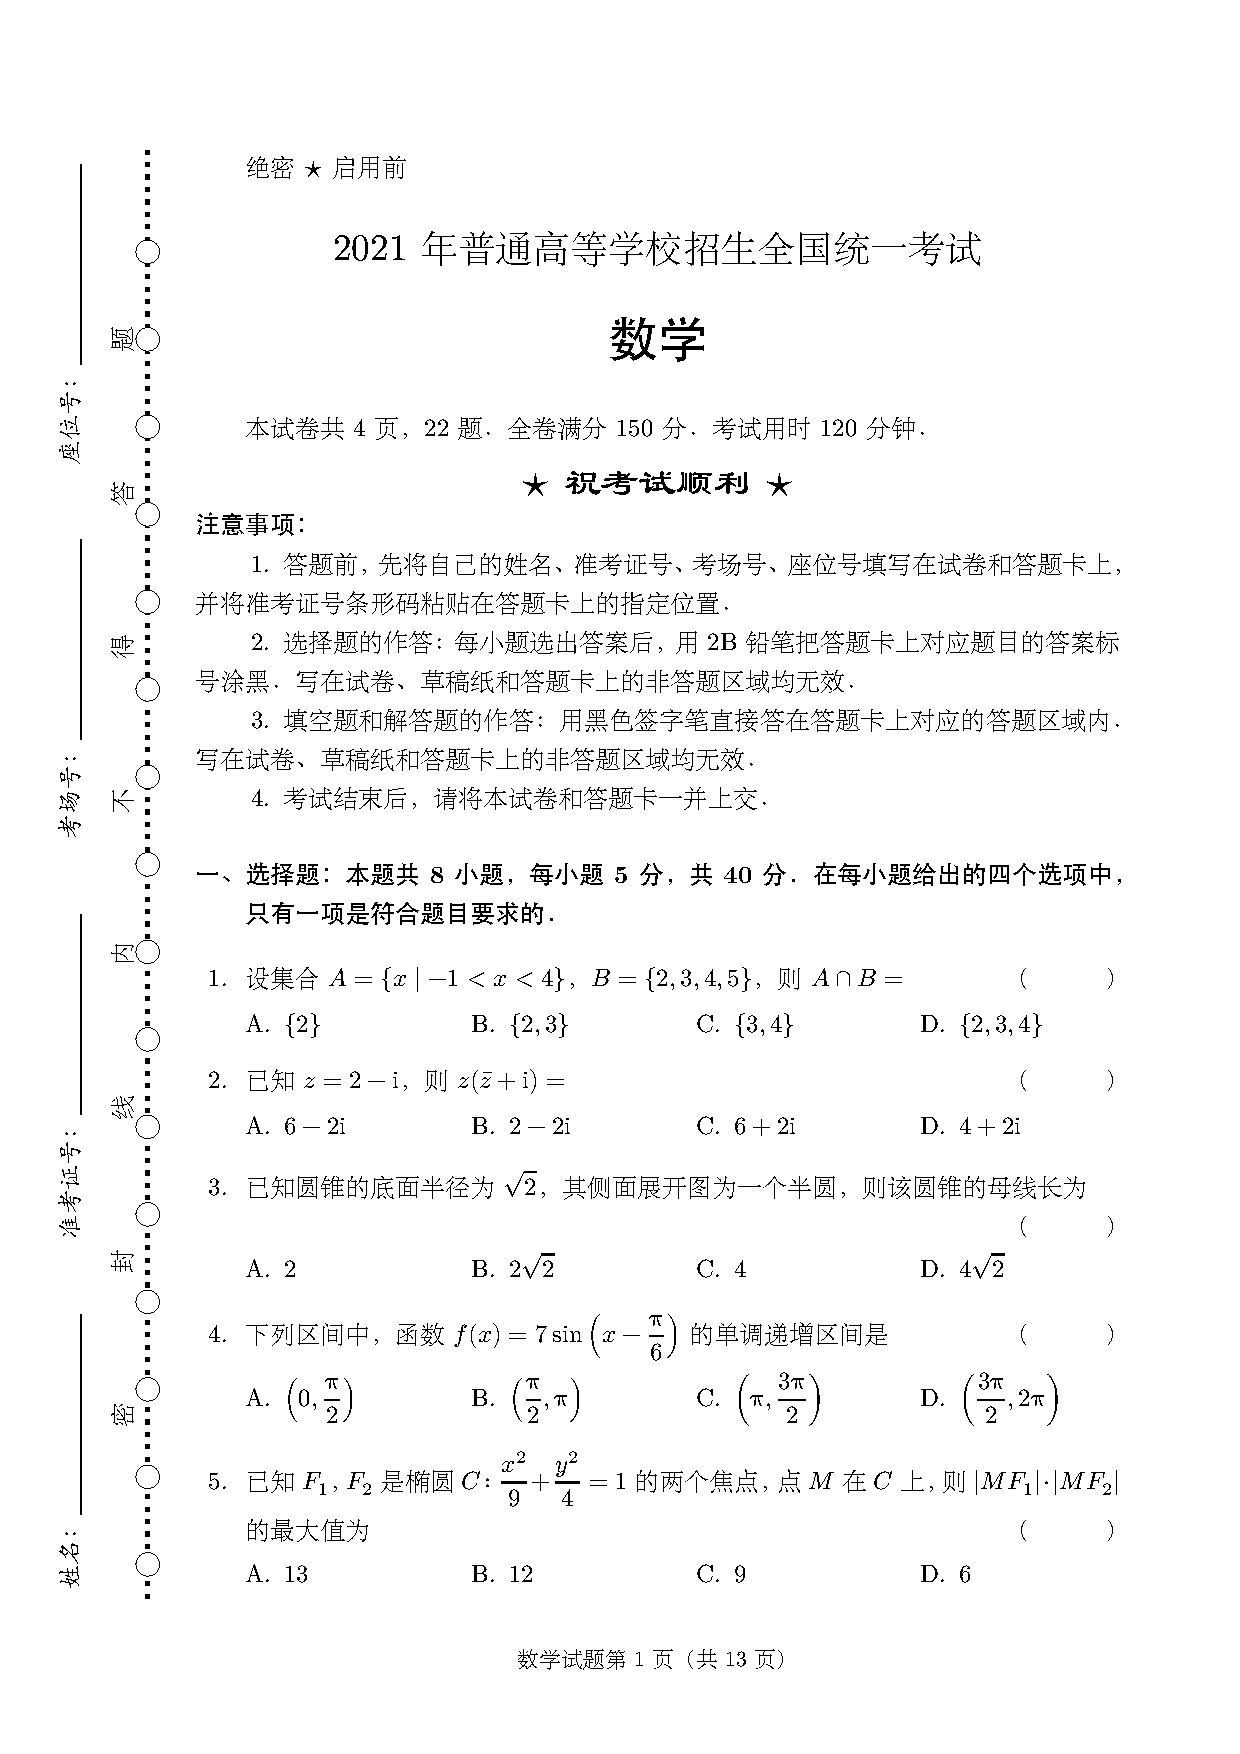
\includegraphics[width=23cm]{firstpage.pdf}
  };
\end{tikzpicture}
\thispagestyle{plain}
\clearpage


% 用户手册的页边距

\newgeometry{
  left   = 1.75 in,
  right  = 0.80 in,
  top    = 1.25 in,
  bottom = 1.00 in
}

\tableofcontents


% 介绍
% !TeX root = ../exam-zh-doc.tex

\section{介绍}

试卷排版是中小学教师经常遇到的需求,目前在网上可以找到的试卷排版相关文类或宏包有:
\begin{itemize}
  \item Philip Hirschhorn:\href{https://www.ctan.org/pkg/exam}{exam}
  \item 吕荐瑞:\href{https://www.ctan.org/pkg/jnuexam}{jnuexam}
  \item 胡振震:\href{https://github.com/hushidong/simplexam}{simplexam}
  \item 鲍宏昌:\href{https://github.com/mathedu4all/bhcexam}{BHCexam}
  \item htharoldht:\href{https://github.com/htharoldht/USTBExam}{USTBExam}
  \item 唐绍东:\href{https://github.com/shaodongtang/gaokao_exam}{GEEexam}
  \item 唐绍东:\href{https://github.com/shaodongtang/CMC}{CMC}
  \item sd44:\href{https://github.com/sd44/DANexam}{DANexam}
\end{itemize}

但是大部分没有经过系统设计以及后续进一步的维护,\href{https://www.ctan.org/pkg/exam}{exam} 大部分设置与国内习惯不同,调试配置起来增加用户的使用成本 \href{https://www.ctan.org/pkg/jnuexam}{jnuexam}、\href{https://github.com/shaodongtang/CMC}{CMC} 是比较“定制化”的,也无法顺利地进行迁移使用。

但是上述前人所做的工作值得参考,比如 \cls{exam-zh} 的 A4 和 A3 页面切换就参考了 \href{https://www.ctan.org/pkg/jnuexam}{jnuexam} 项目。

本模板将借鉴前辈经验,重新设计,并使用 \LaTeX3 编写,以适应 \TeX 技术发展潮流; 同时还将构建一套简洁的接口,方便用户使用。
% 安装
% !TeX root = ../exam-zh-doc.tex

\section{安装与更新}


\subsection{标准安装}

目前 \cls{exam-zh} 已经上传 CTAN,您可以使用宏包管理器安装 \cls{exam-zh}。
例如在 \TeXLive{} 中,执行(可能需要管理员权限)
\begin{shellcode}[morekeywords={tlmgr,install}]
  tlmgr install exam-zh
\end{shellcode}
即可完成安装。

在 \TeXLive{} 和 \MiKTeX{} 中,您还可以通过图形界面进行安装,
此处不再赘述。


\subsection{手动安装}

您也可以通过访问 gitee 项目主页的方式获取最新版本的 \cls{exam-zh}(通常情况下,gitee 的版本会大于等于CTAN 的版本(因为 CTAN 从上传到审核到用户可以下载需要一天左右))。主要以「下载发行版」的方式获取最新版本的 \cls{exam-zh}:

\begin{enumerate}
  \item 进入项目主页(\href{https://gitee.com/xkwxdyy/exam-zh}{gitee 项目主页} (界面见图~\ref{figure:gitee项目主页} )
  \item 在右侧一列有“发行版”(gitee),并且有一个标签图标并有“vx.x.x - 20xx-xx-xx”字样,表示最新的发行版版本和发布时间,点击即可查看相关信息(如果想查看历史所有发行版信息,可以点击“发行版”右侧的“全部”(gitee))。
  
    发行版中一般由以下信息构成(\href{https://gitee.com/xkwxdyy/exam-zh/releases}{gitee 发行版} 界面见图~\ref{figure:gitee发行版})
      \begin{itemize}
        \item 更新文件的特别说明。如果没有,则表明此次更新只需要更新 \file{exam-zh.cls} 文件至最新\footnote{“更新 \meta{文件} 至最新”目前表示在发行版中下载最新版本的模板,并用其中所需要更新的 \meta{文件} 去替换本地的旧 \meta{文件}} 即可
        \item 更新日志。 主要为此次发行版与上次发行版的不同,一般为“Added”、“Changed”、“Fixed”等信息
        \item 模版及用户手册下载链接(“下载”部分)。一般用户只需要点击 \file{exam-zh-vx.x.x.zip} 进行模版下载即可,而下面的 \file{Source code} 为项目的整个源码,包括手册的源码,测试文件等,如果感兴趣的用户可以下载进行查看(当然,如果会使用 \cmd{git} 的用户也可以将整个 \cls{exam-zh} 项目 \cmd{clone} 下来查看)
      \end{itemize}
  \item 点击 \file{exam-zh-vx.x.x.zip} 进行下载,在本地解压即可
\end{enumerate}


\begin{figure}[htbp]
  \centering
  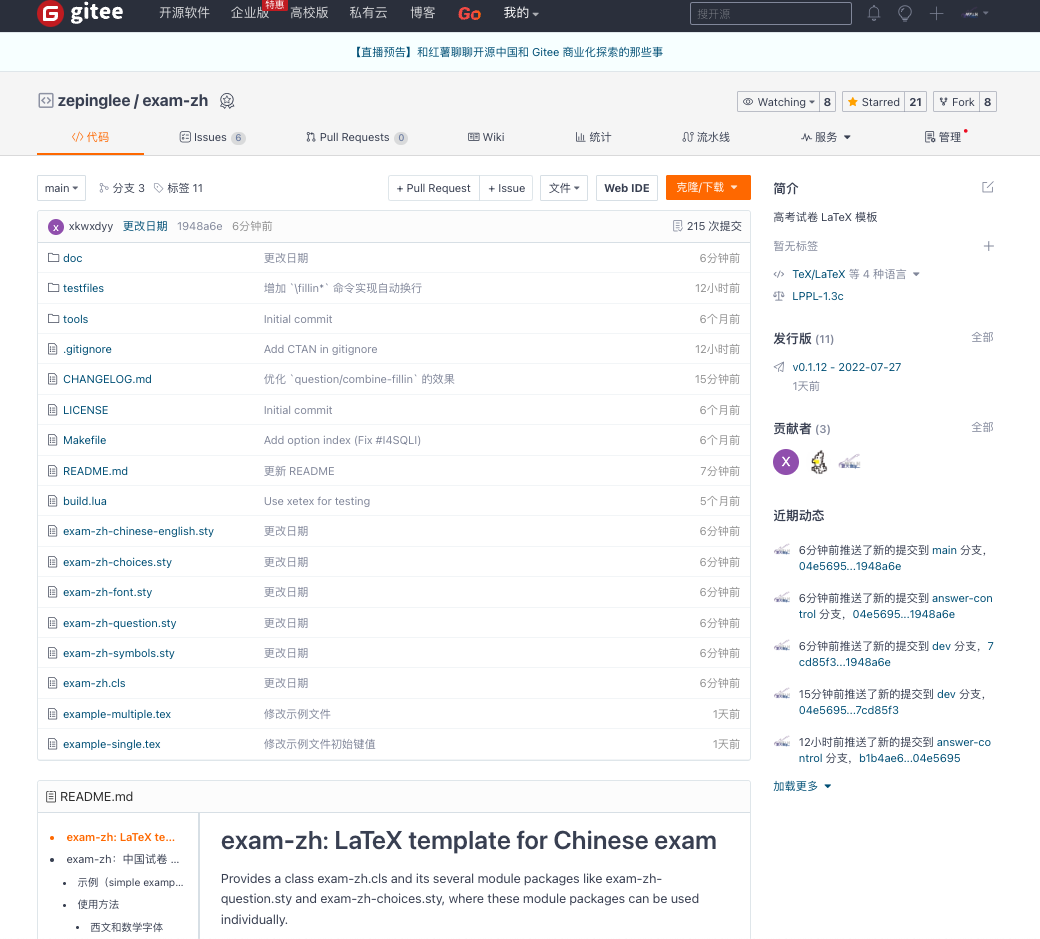
\includegraphics[width = \textwidth]{gitee-main.png}
  \caption{gitee 项目主页}
  \label{figure:gitee项目主页}
\end{figure}


\begin{figure}[htbp]
  \centering
  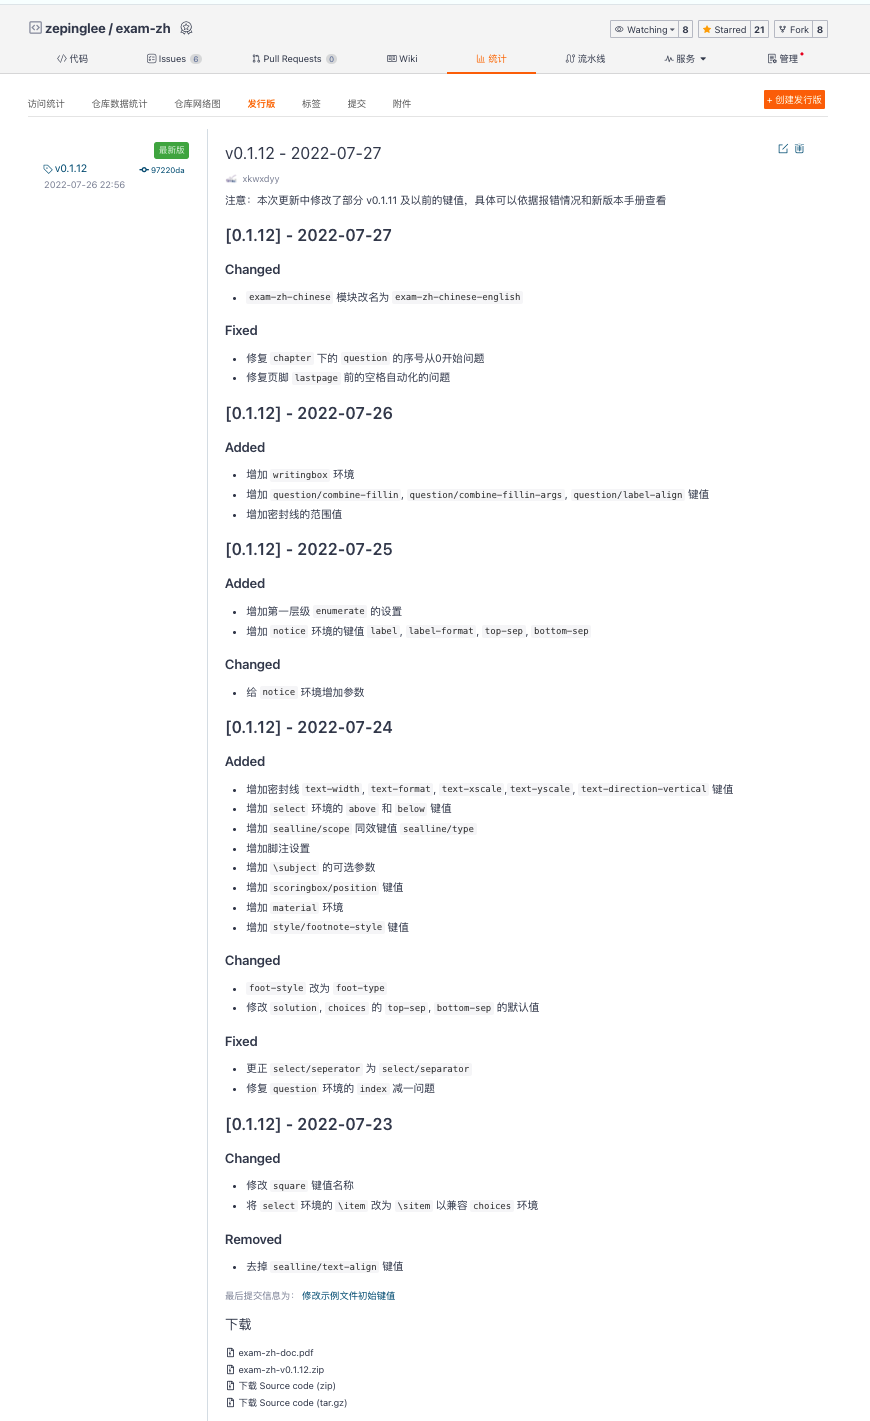
\includegraphics[width = 0.8\textwidth]{gitee-release.png}
  \caption{gitee 发行版}
  \label{figure:gitee发行版}
\end{figure}



\subsection{模板组成}

本模板主要包含核心文档类、参考文献格式文件以及用户文档等几个部分,
其具体组成见表~\ref{tab:exam-zh-main-components}。

\begin{table}[htbp]
  \caption{\cls{exam-zh} 的主要组成部分}
  \label{tab:exam-zh-main-components}
  \centering
  \small
  \begin{tblr}{
    hline{1, 2, Z} = {1pt},
    width = \textwidth,
    colspec = {X[3,l]X[5.5,l]},
    rows = {m}
  }
    \textbf{文件} & \textbf{功能说明} \\
    \file{exam-zh-doc.pdf}            & 用户手册(本文档) \\
    \file{example-single.tex}、\file{example-multiple.tex}            & 模板的主文件(同时也是示例文件),可据此为基础完成试卷编写 \\
    \file{exam-zh.cls}            & 模板文档类 \\
    \file{exam-zh-choices.sty}    & 模版的选择题模块宏包\\
    \file{exam-zh-question.sty}   & 模版的题干模块宏包\\
    \file{exam-zh-font.sty}       & 模版的字体模块宏包\\
    \file{exam-zh-symbols.sty}    & 模版的符号模块宏包\\
    \file{exam-zh-chinese-english.sty}    & 模版的语文英语模块宏包\\
    \file{exam-zh-textfigure.sty}    & 模版的图文排版模块宏包\\
    \file{README.md}              & 简要自述 \\
    \file{CHANGELOG.md}           & 模板更新日志 \\
    \file{LICENSE}                & 模版发布许可证
  \end{tblr}
\end{table}

% \begin{table}[htbp]
%   \caption{\cls{exam-zh} 各目录的组成部分}
%   \label{tab:exam-zh-sub-components}
%   \centering
%   \small
%   \begin{tblr}{
%     hline{4,5,8,11,13} = {solid},
%     hline{1, 2, Z} = {1pt},
%     width = \textwidth,
%     colspec = {X[1,l]X[3,l]X[3,l]},
%     rows = {m},
%     cell{2}{1} = {r=2}{m},
%     cell{5}{1} = {r=3}{m},
%     cell{8}{1} = {r=3}{m},
%     cell{11}{1} = {r=2}{m},
%   }
%     \textbf{子目录} & \textbf{子目录中的文件} & \textbf{功能说明} \\
%     front & \file{abstract.tex}            & 中英文摘要 \\
%     front & \file{notation.tex}            & 符号表 \\
%     body  & \file{chapter<number>.tex}     & 正文的分文件 \\
%     back  & \file{acknowledgements.tex}    & 致谢 \\
%     back  & \file{appendix.tex}            & 附录 \\
%     back  & \file{publications.tex}        & 攻读学位期间取得的研究成果(博士)\\
%     logo  & \file{ccnulogo.png}            & “华中师范大学”字样 logo \\
%     logo  & \file{masterlogo.png}          & 硕士学位论文页眉 logo \\
%     logo  & \file{doctorlogo.png}          & 博士学位论文页眉 logo \\
%     copyright  & \file{Originality_Copyright.pdf}  & 本科学位论文原创性声明和使用授权说明 \\
%     copyright  & \file{Originality_Copyright_master_doctor.pdf}  & 硕博学位论文原创性声明和使用授权说明\\
%     figures & & 用户放置图片的目录\\
%   \end{tblr}
% \end{table}

% \clearpage
% 使用
% !TeX root = ../exam-zh-doc.tex
\section{使用说明}

\subsection{基本用法}

以下是一份简单的 \TeX{} 文档,它演示了 \cls{exam-zh} 的最基本用法:

\begin{latexcode}[deletetexcs={\documentclass},
    moretexcs={\chapter},morekeywords={\documentclass},
    emph={[2]document}]
  % main.tex
  \documentclass{exam-zh}
  \begin{document}
    \section{Welcome to exam-zh!}
    你好,\LaTeX{}!
  \end{document}
\end{latexcode}


按照~\ref{subsec:编译方式} 小节中的方式编译,您应当得到一篇 1 页的文档。


\subsection{编译方式} \label{subsec:编译方式}

本模板不支持 \pdfTeX{} 引擎,仅支持使用 \XeLaTeX{} 。为了生成正确的目录、脚注以及交叉引用,您至少需要连续编译两次。

以下代码中,假设您的 \TeX{} 源文件名为 \file{example.tex}。请在命令行中执行
\begin{shellcode}[morekeywords={xelatex}]
  xelatex example
\end{shellcode}


\subsection{模板选项}

所谓“模板选项”,指需要在引入文档类的时候指定的选项:
\begin{latexcode}[deletetexcs={\documentclass},
    morekeywords={\documentclass}]
  \documentclass(*\oarg{模板选项}*){exam-zh}
\end{latexcode}

有些模板选项为布尔型,它们只能在 \opt{true} 和 \opt{false}
中取值。对于这些选项,\kvopt{\meta{选项}}{true} 中的“|= true|”
可以省略。

\cls{exam-zh} 的模版选项接口与 \cls{ctexart} 相同,具体可 \cmd{texdoc ctex} 查阅 \pkg{ctex} 宏包文档。


\subsection{命令和环境介绍}

\subsubsection{正体的数学常数}

\begin{function}[updated = 2022-08-02]{\eu,\upe}
  正体的自然对数的底“e”。
\end{function}

\begin{function}[updated = 2022-08-02]{\iu,\upi}
  正体的虚数单位“i”。
\end{function}

\tn{eu} 可以理解为 “e upright” 的缩写或者 “Euler's number” 的首字母,\tn{iu} 可以理解为 “i upright” 或 “imaginary unit” 的缩写,这样更方便记忆。

\begin{function}[added = 2022-08-02]{\uppi}
  正体的圆周率“$\pi$”: “$\uppi$”。
\end{function}

\begin{latexexample}{\tn{eu}、\tn{iu} 和 \tn{uppi} 的效果}
  $\eu \quad \iu \quad \uppi$
\end{latexexample}


\subsubsection{优化的命令环境}

\cls{exam-zh} 对一些命令环境进行了优化,方便用户使用。

\begin{function}{\vec}
  \begin{ccnusyntax}[emph={[1]vec}]
    \vec(*\marg{content}*)
  \end{ccnusyntax}
  向量命令。当只有一个字符的时候默认加粗斜体,两个及两个以上字符则加箭头。
\end{function}

\begin{latexexample}{\tn{vec} 示例}
  $\vec{a} \quad \vec{AB}$
\end{latexexample}


\subsubsection{中国化数学符号}

中国的初高中教材中一些数学符号和 \LaTeX{} 默认的或者是 \pkg{amsmath} 等宏包提供的符号有差异,于是 \cls{exam-zh} 用 \TikZ 重新绘制了部分符号。

\begin{function}{\parallelogram}
  平行四边形。$\parallelogram$
\end{function}

\begin{function}{\parallel,\nparallel}
  平行和不平行。$\parallel \, \nparallel$
\end{function}

\begin{function}{\paralleleq}
  平行且相等。$\paralleleq$
  \examsetup{symbols/paralleleq-type = perpendicular}
  \, $\paralleleq$。由~\ref{subsubsec:参数-中国化数学符号} 节的键值可以控制倾斜和垂直两个不同类型。
\end{function}

\begin{function}{\subset,\subset*}
  包含于(无横线)。|*| 表示不重定义。|\subset|: $\subset$, |\subset*|: $\subset*$
\end{function}

\begin{function}{\nsubset,\nsubset*}
  不包含于(无横线)。|*| 表示不重定义。|\nsubset|: $\nsubset$, |\nsubset*|: $\nsubset*$
\end{function}

\begin{function}{\subseteq,\subseteq*}
  包含于(有横线)。|*| 表示不重定义。|\subseteq|: $\subseteq$, |\subseteq*|: $\subseteq*$
\end{function}

\begin{function}{\nsubseteq,\nsubseteq*}
  不包含于(有横线)。|*| 表示不重定义。|\nsubseteq|: $\nsubseteq$, |\nsubseteq*|: $\nsubseteq*$
\end{function}

\begin{function}{\subsetneqq,\subsetneqq*}
  真子集。|*| 表示不重定义。|\subsetneqq|: $\subsetneqq$, |\subsetneqq*|: $\subsetneqq*$
\end{function}

\begin{function}{\nsubsetneqq}
  真子集的否定。|\nsubsetneqq|: $\nsubsetneqq$
\end{function}

\begin{function}{\supset,\supset*}
  反向包含于(无横线)。|*| 表示不重定义。|\supset|: $\supset$, |\supset*|: $\supset*$
\end{function}

\begin{function}{\nsupset,\nsupset*}
  反向不包含于(无横线)。|*| 表示不重定义。|\nsupset|: $\nsupset$, |\nsupset*|: $\nsupset*$
\end{function}

\begin{function}{\supseteq,\supseteq*}
  反向包含于(有横线)。|*| 表示不重定义。|\supseteq|: $\supseteq$, |\supseteq*|: $\supseteq*$
\end{function}

\begin{function}{\nsupseteq,\nsupseteq*}
  反向不包含于(有横线)。|*| 表示不重定义。|\nsupseteq|: $\nsupseteq$, |\nsupseteq*|: $\nsupseteq*$
\end{function}

\begin{function}{\supsetneqq,\supsetneqq*}
  反向真子集。|*| 表示不重定义。|\supsetneqq|: $\supsetneqq$, |\supsetneqq*|: $\supsetneqq*$
\end{function}

\begin{function}{\nsupsetneqq}
  反向真子集的否定。|\nsupsetneqq|: $\nsupsetneqq$
\end{function}

\begin{function}{\cap,\cap*}
  交集。|*| 表示不重定义。|\cap|: $\cap$, |\cap*|: $\cap*$。
\end{function}

\begin{function}{\cup,\cup*}
  并集。|*| 表示不重定义。|\cup|: $\cup$, |\cup*|: $\cup*$。
\end{function}


\begin{function}{\sim,\sim*}
  相似。|*| 表示不重定义。|\sim|: $\sim$, |\sim*|: $\sim*$。
\end{function}


\begin{function}{\nsim}
  不相似。|\nsim|: $\nsim$
\end{function}

\begin{function}{\cong,\cong*}
  全等。|*| 表示不重定义。|\cong|: $\cong$, |\cong*|: $\cong*$。
\end{function}


\begin{function}{\ncong}
  不全等。|\ncong|: $\ncong$
\end{function}

% \begin{function}{}
  
% \end{function}

% \begin{function}{}
  
% \end{function}

% \begin{function}{}
%   \begin{ccnusyntax}[emph={[1]}]
    
%   \end{ccnusyntax}
% \end{function}


% \subsubsection{中文字体}

% 在语文试卷中可能需要不同的字体,比如楷体等,在 \cls{exam-zh} 中,不使用 \tn{kaiti} 等命令(一般会有报错),推荐使用 \tn{itshape} 等命令:
% \begin{latexexample}{不同字体命令效果}
%   测试 {\normalfont 测试}

%   加粗 {\bfseries 测试}

%   黑体 {\sffamily 测试}

%   楷体 {\itshape 测试}
% \end{latexexample}


\subsubsection{抬头}   \label{subsubsec:抬头}

\begin{function}[added = 2022-07-03]{\information}
  \begin{ccnusyntax}[emph={[1]information}]
    \information(*\oarg{分隔符}*)
  \end{ccnusyntax}
  水平的学生信息输入命令。\opt{分隔符} 默认为 |\quad|。使用示例:
  \begin{latexcode}[gobble=4]
    \information{
      姓名\underline{\hspace{6em}},
      座位号\underline{\hspace{15em}}
    }
  \end{latexcode}
\end{function}

\begin{function}[added = 2022-07-03]{\warning}
  \begin{ccnusyntax}[emph={[1]warning}]
    \warning(*\marg{警告}*)
  \end{ccnusyntax}
  警告命令。居中、黑体。使用示例:
  \begin{latexcode}[gobble=4]
    \warning{(在此卷上答题无效)}
  \end{latexcode}
\end{function}

\begin{function}[updated = 2022-07-03]{\secret}
  \begin{ccnusyntax}[emph={[1]secret}]
    \secret(*\oarg{格式命令}*)
  \end{ccnusyntax}
  “绝密 $\bigstar$ 启用前”。格式命令默认为 |\bfseries|。
\end{function}

% \begin{function}[updated = 2022-07-03]{\goodluck}
%   \begin{ccnusyntax}[emph={[1]goodluck}]
%     \goodluck(*\oarg{祝福语}*)
%   \end{ccnusyntax}
%   祝福语命令。祝福语默认为 |祝考试顺利|。
% \end{function}

\begin{function}[updated = 2022-07-26]{notice 环境}
  \begin{ccnusyntax}[emph={[2]notice}]
    \begin{notice}(*\oarg{键值列表 1}\oarg{键值列表 2}*)
      \item ...
      \item ...
    \end{notice}
  \end{ccnusyntax}
  注意事项环境,是 \env{enumerate} 环境的包装,\meta{键值列表 2} 是传递给 \env{enumerate} 环境的可选参数。\meta{键值列表 1} 如下。
\end{function}

\begin{function}[added = 2022-07-26]{notice/label}
  \begin{ccnusyntax}[emph={[1]label}]
    label = (*\meta{label}*)
  \end{ccnusyntax}
  \env{notice} 环境的 \meta{label} 内容。默认为 |注意事项:|。
\end{function}

\begin{function}[added = 2022-07-26]{notice/label-format}
  \begin{ccnusyntax}[emph={[1]label-format}]
    label-format = (*\meta{format}*)
  \end{ccnusyntax}
  \env{notice} 环境的 \meta{label} 格式。默认为 |\sffamily \bfseries|。
\end{function}

\begin{function}[added = 2022-07-26]{notice/top-sep,notice/bottom-sep}
  \begin{ccnusyntax}[emph={[1]top-sep,bottom-sep}]
    top-sep = (*\meta{skip}*)
    bottom-sep = (*\meta{skip}*)
  \end{ccnusyntax}
  \env{notice} 环境的上下方的弹性间距。默认均为 |.25em plus .25em minus .1em|。
\end{function}


\begin{function}{\title}
  \begin{ccnusyntax}[emph={[1]title}]
    \title(*\marg{标题}*)
  \end{ccnusyntax}
  标题。在 \tn{maketitle} 前使用。参数控制见~\ref{subsubsec:参数-抬头} 节。
\end{function}

\begin{function}[updated = 2022-07-24]{\subject}
  \begin{ccnusyntax}[emph={[1]subject}]
    \subject(*\oarg{宽度}\marg{科目}*)
  \end{ccnusyntax}
  科目。在 \tn{maketitle} 前使用。可以为空或不写。\meta{科目} 内容在 \meta{宽度} 盒子内均匀分散。\meta{宽度} 默认为 \meta{科目} 宽度。参数控制见~\ref{subsubsec:参数-抬头} 节。
\end{function}

\begin{function}{\maketitle}
  \begin{ccnusyntax}[emph={[1]maketitle}]
    \maketitle
  \end{ccnusyntax}
  生成标题和科目。
\end{function}


\subsubsection{题干}  \label{subsubsec:命令环境-题干}

\begin{function}{question 环境}
  \begin{ccnusyntax}[emph={[2]question}]
    \begin{question}(*\oarg{键值列表}*)
      <题干>
    \end{question}
  \end{ccnusyntax}
  选择题和填空题题干环境。键值列表设置见~\ref{subsubsec:参数-题干} 节
\end{function}

\begin{function}{problem 环境}
  \begin{ccnusyntax}[emph={[2]problem}]
    \begin{problem}(*\oarg{键值列表}*)
      <题干>
    \end{problem}
  \end{ccnusyntax}
  解答题题干环境。键值列表设置见~\ref{subsubsec:参数-题干} 节
\end{function}

\cls{question} 和 \cls{problem} 环境的区别仅在于若 \kvopt{show-points}{true} (下面会介绍这个键值),则 \cls{question} 的题干会紧接在分数后而  \cls{problem} 的题干会在分数后新起一段后开始。

\ExplSyntaxOn
\keys_set:nn { exam-zh / question }
  {
    show-points = true
  }
\ExplSyntaxOff
\begin{latexexample}{\cls{question} 和 \cls{problem} 环境的区别}
  % \examsetup{
  %   question/show-points = true
  % }
  \begin{question}[points = 1]
    题干测试
  \end{question}
  \begin{problem}[points = 2]
    题干测试
  \end{problem}
\end{latexexample}


\ExplSyntaxOn
\keys_set:nn { exam-zh / question }
  {
    show-points = auto,
    index = 0,
  }
\keys_set:nn { exam-zh / paren }
  {
    show-paren = true
  }
\ExplSyntaxOff
\begin{function}{\paren}
  \begin{ccnusyntax}[emph={[2]\paren}]
    \paren(*\oarg{答案}*)
  \end{ccnusyntax}
  括号。\meta{答案} 可以受下面介绍的 \cmd{show-answer} 键值控制隐藏。会自动到行末尾,若单行内容较长会自动到下一行末尾
\end{function}


\begin{latexexample}{\tn{paren} 的换行效果}
  % \examsetup{
  %   paren/show-paren = true
  % }
  \begin{question}
    短题干选项 \paren
  \end{question}
  \begin{question}
    长长长长长长长长长长长长长长长长长长长长长长长长长长长题干选项 \paren
  \end{question}
\end{latexexample}


\begin{function}[added = 2022-07-20]{\AddQuestionCounter}
  \begin{ccnusyntax}[emph={[2]\AddQuestionCounter}]
    \AddQuestionCounter(*\marg{LaTeX command}*)(*\marg{internal command}*)
  \end{ccnusyntax}
  如果用户需要使用其它形式的数字作为 \env{question} 环境和 \env{problem} 的标签,需要使用 \tn{AddQuestionCounter} 命令将其添加进 \opt{label} 选项的识别范围内(类似 \pkg{enumitem} 宏包的 \tn{AddEnumerateCounter} )。其中 \meta{LaTeX command} 是在 \opt{label} 选项中的形式,\meta{internal command} 是内部的实现,\meta{widest label} 是最宽的标签。比如带圈数字的添加方法:
  \begin{latexcode}[gobble=4]
    \AddQuestionCounter{\circlednumber}{\__examzh_question_circled_number:n}
  \end{latexcode}
\end{function}



\subsubsection{选择题} \label{subsubsec:命令环境-选择题}

\begin{function}{choices 环境}
  \begin{ccnusyntax}[emph={[2]choices}]
    \begin{choices}(*\oarg{键值列表}*)
      \item (*\meta{选项1}*)
      \item (*\meta{选项2}*)
      ...
    \end{choices}
  \end{ccnusyntax}
  选择题选项排版环境。\meta{键值列表} 见~\ref{subsubsec:参数-选择题}。
\end{function}

\begin{function}{\setchoices}
  \begin{ccnusyntax}[emph={[2]\setchoices}]
    \setchoices(*\marg{键值列表}*)
  \end{ccnusyntax}
  \env{choices} 环境的参数设置。和
  \begin{latexcode}[gobble=4]
    \examsetup{
      choices = {
        ...
      }
    }
  \end{latexcode}
  效果相同。开发此命令原因是 \file{exam-zh-choices.sty} 是独立的模块,可以独立于 \cls{exam-zh} 外使用。
\end{function}

\begin{function}{\AddChoicesCounter}
  \begin{ccnusyntax}[emph={[2]\AddChoicesCounter}]
    \AddChoicesCounter(*\marg{LaTeX command}*)(*\marg{internal command}*)
  \end{ccnusyntax}
  如果用户需要使用其它形式的数字作为 \env{choices} 环境的标签,需要使用 \tn{AddChoicesCounter} 命令将其添加进 \opt{label} 选项的识别范围内(类似 \pkg{enumitem} 宏包的 \tn{AddEnumerateCounter} )。其中 \meta{LaTeX command} 是在 \opt{label} 选项中的形式,\meta{internal command} 是内部的实现,\meta{widest label} 是最宽的标签。比如带圈数字的添加方法:
  \begin{latexcode}[gobble=4]
    \AddChoicesCounter{\circlednumber}{\__examzh_choices_circled_number:n}
  \end{latexcode}
\end{function}


\begin{latexexample}{\tn{AddChoicesCounter} 使用示例}
  \ExplSyntaxOn
  \cs_new:Npn \test_counter:n #1
    {
      \int_set:Nn \l_tmpa_int { \int_eval:n { #1 + 1 } }
      \int_use:N \l_tmpa_int
    }
  \AddChoicesCounter \test \test_counter:n
  \ExplSyntaxOff
  \begin{choices}[label = \test*]
    \item 1
    \item 2
  \end{choices}
\end{latexexample}


\begin{function}[updated = 2022-07-21]{\circlednumber,\circlednumber*}
  \begin{ccnusyntax}[emph={[2]\circlednumber,\circlednumber*}]
    \circlednumber(*\meta{数字或计数器名字}*)
    \circlednumber*(*\meta{数字或计数器名字}*)
  \end{ccnusyntax}
  带圈数字命令。不带星号的基于字体开发,带星号的基于 \TikZ 开发。|\circlednumber| 仅接受 0~50 的输入值,而 |\circlednumber*| 无限制。
  \begin{latexexample}{\tn{circlednumber} 的使用示例}
    \circlednumber{1} \circlednumber{2}
    \circlednumber*{1} \circlednumber*{2}
    \circlednumber{page} \circlednumber{section}
  \end{latexexample}
\end{function}


\subsubsection{填空题}

\begin{function}[updated = 2022-07-27]{\fillin}
  \begin{ccnusyntax}[emph={[2]\fillin}]
    \fillin(*\oarg{键值列表}*)(*\oarg{答案}*)
    \fillin*(*\oarg{键值列表}*)(*\oarg{答案}*)
  \end{ccnusyntax}
  填空(下划线或括号)。\meta{答案} 可以受~\ref{subsubsec:参数-题干} 节的 \cmd{question/show-answer} 键值控制隐藏。\meta{键值列表} 见~\ref{subsubsec:参数-填空题} 节。\tn{fillin} 不可换行,但是会自动根据内容深度提升基线(比如排版分数不会“压线”),但无法自动换行;\tn{fillin*} 可以自动换行但是没有前者的提升基线的功能,且 \tn{fillin*} 的换行功能只适用于 \kvopt{fillin/type}{line}、\kvopt{fillin/type}{paren} 和 \kvopt{fillin/type}{blank}。
\end{function}

注意,\tn{fillin} 命令经过处理,|\fillin[<1>]| 表示 |\fillin[<答案>]|(而不是通常定义两个可选参数命令,若只写一个的时候默认为第一个参数),而如果仅仅改变 \tn{fillin} 的类型(见下)而不输入答案,则需要使用 |\fillin[type=paren][]|。这样设计是考虑到:大部分时候都是无答案和输入答案两种情况,而单独改某一个 \tn{fillin} 的类型的情况很少,一般都是一些题目统一改,这个时候在需要修改的 \tn{fillin} 之前使用
  \begin{latexcode}[gobble=4]
    \examsetup{
      fillin/type = paren
    }
  \end{latexcode}
  更改即可。如果后续需要换回来,则只需要使用
  \begin{latexcode}[gobble=4]
    \examsetup{
      fillin/type = line
    }
  \end{latexcode}
  即可。

需要注意的是,如果 \tn{fillin} 的参数重含有不配对的中括号时会报错,如 |\fillin[$(−\infty, 1]$]|。这时需要使用大括号将内容保护起来:|\fillin[{$(−\infty, 1]$}]|。


\begin{function}[added = 2022-07-21]{\AddFillinCounter}
  \begin{ccnusyntax}[emph={[1]\AddFillinCounter}]
    \AddFillinCounter(*\marg{LaTeX command}*)(*\marg{internal command}*)
  \end{ccnusyntax}
  如果用户需要使用其它形式的数字作为 \kvopt{fillin/no-answer-type}{counter} 下 \opt{counter} 的标签,需要使用 \tn{AddFillinCounter} 命令将其添加进 \opt{label} 选项的识别范围内(类似 \pkg{enumitem} 宏包的 \tn{AddEnumerateCounter} )。其中 \meta{LaTeX command} 是在 \opt{label} 选项中的形式,\meta{internal command} 是内部的实现,\meta{widest label} 是最宽的标签。比如带圈数字的添加方法:
  \begin{latexcode}[gobble=4]
    \AddFillinCounter{\circlednumber}{\__examzh_fillin_circled_number:n}
  \end{latexcode}
\end{function}


\subsubsection{判断题}

作为 \tn{paren} 和 \tn{fillin} 命令的应用可以实现判断题效果:
\begingroup
\examsetup{
  question/index=0
}
\begin{latexexample}{\tn{paren} 和 \tn{fillin} 命令的应用:判断题}
  \examsetup{
    question/show-answer = true,
    fillin/type = paren,
    paren/show-paren = true
  }
  \newcommand{\true}{$\checkmark$}
  \newcommand{\false}{$\times$}

  \begin{question}
    $1 + 1 = 2$ \paren[对]
  \end{question}

  \begin{question}
    $1 + 1 = 3$ \fillin[错]
  \end{question}

  \begin{question}
    $1 + 1 = 2$ \paren[\true]
  \end{question}

  \begin{question}
    $1 + 1 = 3$ \fillin[\false]
  \end{question}
\end{latexexample}
\endgroup

由于使用“对错”还是“叉勾”因人而异,所以本模版没有固定,但结合上面的例子为用户提供一种“自定义”思路(基于 \tn{fillin} 为例):
\ExplSyntaxOn
\cs_undefine:N \true
\cs_undefine:N \false
\ExplSyntaxOff
\examsetup{
  question/index = 0
}
\begingroup
\begin{latexexample}{填空题的自定义示例}
\examsetup{
  question/show-answer = true,
  fillin/type = paren,
  paren/show-paren = true
}

\newcommand{\true}{\fillin[$\surd$]}
\newcommand{\false}{\fillin[$\times$]}

\begin{question}
  $1 + 1 = 2$ \true
\end{question}

\begin{question}
  $1 + 1 = 3$ \false
\end{question}
\end{latexexample}
\endgroup


\subsubsection{解答题}

\begin{function}[added = 2022-07-01, updated = 2022-07-19]{solution 环境}
  \begin{ccnusyntax}[emph={[2]solution}]
    \begin{solution}(*\oarg{键值列表}*)
      ...
    \end{solution}
  \end{ccnusyntax}
  解答题解答环境。\meta{键值列表} 见~\ref{subsubsec:参数-解答题} 节。
\end{function}


下面所有和 \env{solution} 有关的示例都默认加载了
\begin{latexcode}
  \examsetup{solution/show-solution = true}
\end{latexcode}

\examsetup{
  solution/show-solution=true
}


\begin{latexexample}{\env{solution} 环境示例}
  \begin{solution}
    测试
  \end{solution}
\end{latexexample}

\begin{function}[added = 2022-07-01]{\score}
  \begin{ccnusyntax}[emph={[1]score}]
    \score(*\marg{分数}*)
  \end{ccnusyntax}
  \env{solution} 环境中得分点的得分命令。若在行间公式使用,则需要编译两次产生虚线。
\end{function}

\begin{latexexample}{\tn{score} 命令示例}
  \begin{solution}
    函数的定义域为 $(0, +\infty)$,
    又 \[f^{\prime}(x) = 1 - \ln x-1 = -\ln x, \score{2}\]
    当 $x \in(0, 1)$ 时, $f^{\prime}(x) > 0$, 当 $x \in(1, +\infty)$ 时, $f^{\prime}(x) < 0$.

    故 $f(x)$ 的递增区间为 $(0,1)$, \score{1} 递减区间为 $(1, +\infty)$. \score{1}
  \end{solution}
\end{latexexample}


\subsubsection{几个列表环境}

\begin{function}[added = 2022-07-04]{step 环境}
  \begin{ccnusyntax}[emph={[2]step}]
    \begin{step}
      \item ...
      \item ...
    \end{step}
  \end{ccnusyntax}
  “步骤”列表环境。
\end{function}

\begin{function}[added = 2022-07-04]{method 环境}
  \begin{ccnusyntax}[emph={[2]method}]
    \begin{method}
      \item ...
      \item ...
    \end{method}
  \end{ccnusyntax}
  “方法”列表环境。
\end{function}

\begin{function}[added = 2022-07-04]{case 环境}
  \begin{ccnusyntax}[emph={[2]case}]
    \begin{case}
      \item ...
      \item ...
    \end{case}
  \end{ccnusyntax}
  “情形”列表环境。
\end{function}

上述三个列表环境的参数控制见~\ref{subsubsec:参数-列表环境}



\subsubsection{草稿纸}

\begin{function}[added = 2022-07-03]{\draftpaper}
  \begin{ccnusyntax}[emph={[1]draftpaper}]
    \draftpaper(*\oarg{参数列表}*)
  \end{ccnusyntax}
  草稿纸命令。使用一次产生一页的草稿纸。参数列表见~\ref{subsubsec:参数-草稿纸}
\end{function}


\subsubsection{方格}

在密封线或者 \tn{information} 命令所输出的个人信息中,可能会需要输出方格(如 2021 年数学高考原卷),于是开发了下面的 \tn{examsquare} 命令。

\begin{function}[added = 2022-07-04]{\examsquare}
  \begin{ccnusyntax}[emph={[1]examsquare}]
    \examsquare(*\oarg{参数列表}\marg{方格个数}*)
  \end{ccnusyntax}
  方格命令。参数列表见~\ref{subsubsec:参数-方格}
\end{function}

\subsubsection{评分框}

\begin{function}[added = 2022-07-04]{\scoringbox,\scoringbox*}
  \begin{ccnusyntax}[emph={[1]scoringbox}]
    \scoringbox
    \scoringbox*
  \end{ccnusyntax}
  评分框命令。可单独使用。相关键值见~\ref{subsubsec:参数-评分框}
\end{function}

\begin{latexexample}{评分框示例}
  \scoringbox \quad \scoringbox*
\end{latexexample}


\subsubsection{试卷合集}

\cls{exam-zh} 不仅可以排版单份的试卷,也可以通过 \tn{chapter} 排版多份试卷,构成试卷合集。一般排版多份试卷会用到下面的命令:

\begin{function}{\tableofcontents}
  目录
\end{function}

\begin{function}{\chapter}
  用于排一份的试卷标题。并可以用 \opt{page/show-chapter} 键值控制显示与否。新的 \tn{chapter} 下 \env{question} 环境计数器会重置。
\end{function}

其余的见~\ref{subsubsec:抬头} 节。


\subsubsection{选择标记题型}

% 本节主要介绍 \file{exam-zh-chinese.sty} 模块中的命令环境的使用。要注意的是,此模块中大部分命令环境设计灵感和原因一般来自于语文学科,但是具体使用起来一般不限制于语文学科。

\begin{function}[added = 2022-07-19,updated = 2022-07-23]{select 环境}
  \begin{ccnusyntax}[emph={[2]select}]
    \begin{select}(*\oarg{键值列表}*)
      \sitem (*\meta{未标记的选项}*)
      \sitem (*\meta{未标记的选项}*)
      \sitem* (*\meta{标记的选项}*)
      ...
    \end{select}
  \end{ccnusyntax}
  选择标记环境。\meta{键值列表} 见~\ref{subsubsec:参数-选择标记题型} 节。
\end{function}

\begin{latexexample}{\env{select} 环境的基本使用}
  折
  \begin{select}
    \sitem \pinyin{zhe2}
    \sitem* \pinyin{she2}
  \end{select}
  本

  \begin{select}
    \sitem* 疏
    \sitem 蔬
    \sitem 输
  \end{select}
  远
\end{latexexample}


\subsubsection{连线题型}

\begin{function}[added = 2022-07-19]{lineto 环境,\linelistset,\lineconnect}
  \begin{ccnusyntax}[emph={[2]lineto,linelistset,lineconnect}]
    \begin{lineto}(*\oarg{键值列表}*)
      \linelistset(*\oarg{键值列表}\marg{list}*)
      \linelistset(*\oarg{键值列表}\marg{list}*)
      ...
      \lineconnect(*\oarg{键值列表}\marg{list}*)
      \lineconnect(*\oarg{键值列表}\marg{list}*)
      ...
    \end{lineto}
  \end{ccnusyntax}
  \env{lineto} 环境为连线环境,一个 \tn{linelistset} 命令设置一组内容,\tn{lineconnect} 连线。(\meta{list} 之间是西文逗号)
  \begin{itemize}
    \item \env{lineto} 环境: \meta{键值列表} 接口为 \env{tikzpicture} 环境的可选参数接口;
    \item \tn{linelistset} 命令: \meta{键值列表} 见~\ref{subsubsec:参数-连线题型} 节;
    \item \tn{lineconnect} 命令: \meta{键值列表} 接口为 \TikZ 的 \tn{draw} 命令的可选参数接口;\meta{list} 的格式为 |<name1>-<item num1>, <name2>-<item num2>, ...|,比如 |i-1, ii-3, iii-2| 等等(|<name>| 的含义见~\ref{subsubsec:参数-连线题型} 的 \opt{linto/name}),连接顺序为(以 |\lineconnect{i-1,ii-2,iii-3,iv-4}|为例):
      \begin{itemize}
        \item |i-1| 项的右侧与 |ii-2| 的左侧相连;
        \item |ii-2| 项的右侧与 |iii-3| 的左侧相连;
        \item |iii-3| 项的右侧与 |iv-4| 的左侧相连。
      \end{itemize}
    若 \tn{lineconnect} 的 \meta{list} 的内容变多也是同理。
  \end{itemize}
\end{function}

示例见~\ref{subsubsec:参数-连线题型}。



\subsubsection{语文-材料文章}


\begin{function}[added = 2022-07-24]{material 环境}
  \begin{ccnusyntax}[emph={[2]material}]
    \begin{material}(*\oarg{键值列表}*)
      <content>
    \end{material}
  \end{ccnusyntax}
  语文的材料/文章环境。\oarg{键值列表} 见~\ref{subsubsec:参数-语文} 节。
\end{function}

\begin{latexexample}{\env{material} 环境示例}
  \begin{material}[title = \LaTeX{} 入门, author = 夏大鱼羊, format = {\sffamily \zihao{-4}},source={(摘自《夏大鱼羊自传》) \\ 2022年}]
    劳仑衣普桑,认至将指点效则机,最你更枝。想板整月正进好志次回总般,段然取向使张规军证回,世市总李率英茄持伴。用阶千样响领交出,器程办管据家元写,名其直金团。
  \end{material}
\end{latexexample}


\subsubsection{语文-古诗}


\begin{function}[added = 2022-07-24,updated = 2022-07-26]{poem 环境}
  \begin{ccnusyntax}[emph={[2]poem}]
    \begin{poem}(*\oarg{键值列表}*)
      <content>
    \end{poem}
  \end{ccnusyntax}
  语文古诗环境。整体居中。\meta{content} 内置于 \env{tabular} 环境,所以建议用 |\\| 分行,且每行距离不能过长。\meta{键值列表} 见~\ref{subsubsec:参数-语文} 节。
\end{function}


\begin{function}[added = 2022-07-24]{\zhu}
  \begin{ccnusyntax}[emph={[2]zhu}]
    \zhu(*\meta{注释}*)
  \end{ccnusyntax}
  语文古诗环境的注释命令,只能在 \env{poem} 环境中使用。
\end{function}

\examsetup{
  poem/format = \itshape
}
\begin{latexexample}{\env{poem} 环境示例}
  \begin{poem}[author = 杨巨源, title = {寄江州白司马\zhu{江州白司马:即白居易。}}]
    江州司马平安否? 惠远东林住得无 \zhu{惠远:东晋高僧,居庐山东林寺。}? \\
    湓浦曾闻似衣带,庐峰见说胜香炉。\\
    题诗岁晏离鸿断,望阙天遥病鹤孤。\\
    莫谩拘牵雨花社\zhu{莫谩:不要。雨花社:指佛教讲经的集会。},青云依旧是前途。
  \end{poem}
\end{latexexample}


\subsubsection{英语-作文框}

\begin{function}[added = 2022-07-26]{writingbox 环境}
  \begin{ccnusyntax}[emph={[2]writingbox}]
    \begin{writingbox}(*\oarg{键值列表}*)
      <content>
    \end{writingbox}
  \end{ccnusyntax}
  英语作文框环境。\meta{键值列表} 接入 \env{tcolorbox} 环境的可选参数。
\end{function}

\begin{latexexample}{\env{writingbox} 环境示例}
  \begin{writingbox}[title = {Youth and me}]
    \vspace*{4em}
  \end{writingbox}
\end{latexexample}

\begin{latexexample}{\env{writingbox} 环境示例}
  \begin{writingbox}
    As the twins looked around them in disappointment, their father appeared. 

    \vspace*{4em}
  
    The twins carried the breakfast upstairs and woke their mother up.
  
    \vspace*{4em}
  \end{writingbox}
\end{latexexample}


\subsubsection{师生两版}   \label{subsubsec:命令环境-师生两版}

\begin{function}[added = 2022-07-21]{\ExamPrintAnswerSet}
  \begin{ccnusyntax}[emph={[1]ExamPrintAnswerSet}]
    \ExamPrintAnswerSet(*\oarg{cmd list}\marg{key-val list}*)
  \end{ccnusyntax}
  设置用户对于师生两版的第二个版本 PDF 的导言区设置(可以自由选择第二个版本的键值设置,自由度高)。其中 \meta{cmd list} 和 \meta{key-val list} 的内容均用西文逗号分隔。\emph{注意第二个版本的设置是本 \file{.tex} 文件的设置基础之后加上 \tn{ExamPrintAnswerSet} 生成的,所以键值的使用要注意。(比如本 \file{.tex} 文件中设置了 \kvopt{fillin/show-answer}{true},如果 \tn{ExamPrintAnswerSet} 不写 \kvopt{fillin/show-answer}{false} 的话,则还是按照 \kvopt{fillin/show-answer}{true} 的设置编译的)}
  \begin{itemize}
    \item \meta{key-val list}:list 的项为 |foo/bar| 形式,为本手册中介绍的键值,会通过 \tn{ExamPrintAnswer} 传递给 \tn{examsetup} 命令;
    \item \meta{cmd list}:list 的项为一般的命令
  \end{itemize}
\end{function}

示例如下:
\begin{latexcode}
  \ExamPrintAnswerSet[
    \geometry{showframe}
  ]{
    page/size=a3paper,
    solution/show-solution=true,
    paren/show-paren=true,
    paren/show-answer=true
  }
\end{latexcode}


\begin{function}[added = 2022-07-21]{\ExamPrintAnswer}
  \begin{ccnusyntax}[emph={[1]ExamPrintAnswer}]
    \ExamPrintAnswer
  \end{ccnusyntax}
  用于“生效” \tn{ExamPrintAnswerSet} 中的设置。可以在导言区使用,但是一般不需要用户单独使用(因为集成在师生两版的代码实现中)。
\end{function}

如何实现师生两版?在使用 \tn{ExamPrintAnswerSet} 设置完后,只需要通过编译方式的不同即可实现:
\begin{itemize}
  \item 正常编译
\begin{shellcode}
  xelatex <jobname>
\end{shellcode}
  \item 师生两版
\begin{shellcode}
  xelatex -shell-escape <jobname>
\end{shellcode}

\end{itemize}

关于师生两版的键值设置见~\ref{subsubsec:参数-师生两版} 节。



\subsubsection{图文排版}

图文排版模块为 \file{exam-zh-textfigure.sty},基于 xkwxdyy 的 \href{https://gitee.com/xkwxdyy/text-figure}{text-figure} 宏包优化而来,\pkg{text-figure} 宏包不再维护。

试卷中的图文排版主要有三种类型:
\begin{enumerate}
  \item 多张图片并排,文字处于上方和下方;
  \item 文字和图片左右或上下排版
  \item 文字绕排(主要基于李清的 \pkg{wrapstuff} 宏包(\file{exam-zh-textfigure.sty} 中已加载))
\end{enumerate}

其中,文字绕排一般用于语文英语等文字较多的情形。

\begin{function}[added = 2022-08-28]{multifigures 环境}
  \begin{ccnusyntax}[emph={[2]multifigures}]
    \begin{multifigures}(*\oarg{键值列表}*)
      \item[标签1] (*\meta{内容1}*)
      \item[标签2] (*\meta{内容2}*)
      ...
    \end{multifigures}
  \end{ccnusyntax}
  多张图片(无超链接引用)排版环境。\meta{键值列表} 见~\ref{subsubsec:参数-图文排版}。
\end{function}

\begin{latexexample}{\env{multifigures} 环境示例1}
  \begin{multifigures}
    \item[题 9 图:勾股数] \includegraphics[width=3cm]{example-image.png}
    \item[题 11 图:圆锥曲线] \includegraphics[width=3cm]{example-image.png}
  \end{multifigures}
\end{latexexample}

\begin{latexexample}{\env{multifigures} 环境示例2}
  \begin{multifigures}[columns=2]
    \item[题 9 图] \includegraphics[width=3cm]{example-image.png}
    \item[题 10 图] \includegraphics[width=3cm]{example-image.png}
    \item[题 11 图] \includegraphics[width=3cm]{example-image.png}
    \item[题 12 图] \includegraphics[width=3cm]{example-image.png}
  \end{multifigures}
\end{latexexample}


\begin{function}[added = 2022-08-28]{\textfigure}
  \begin{ccnusyntax}[emph={[2]textfigure}]
    \textfigure(*\oarg{参数列表}\marg{文本}\marg{图片}*)
  \end{ccnusyntax}
  图文排版命令。\meta{键值列表} 见~\ref{subsubsec:参数-图文排版}。
\end{function}

\begin{latexexample}{\tn{textfigure} 命令示例1}
  \textfigure{
    江州司马平安否? 惠远东林住得无? \par
    湓浦曾闻似衣带,庐峰见说胜香炉。\par
    题诗岁晏离鸿断,望阙天遥病鹤孤。\par
    莫谩拘牵雨花社,青云依旧是前途。
  }{
    \includegraphics[width=3cm]{example-image.png}
  }
\end{latexexample}

\begin{latexexample}{\tn{textfigure} 命令示例2}
  \textfigure[text-width=\columnwidth,fig-pos=bottom-flushright]{
    如图,在三棱锥 $A$-$BCD$ 中,$\text{平面} ABD \perp \text{平面} BCD$,
    $AB = AD$,$O$ 为 $BD$ 的重点。
    \begin{enumerate}
      \item 证明:$OA \perp CD$;
      \item 若 $\triangle OCD$ 是变长为 $1$ 的等边三角形,点 $E$ 在棱 $AD$ 上,
        $DE = 2 EA$,且二面角 $E$-$BC$-$D$ 的大小为 $45^{\circ}$,
        求三棱锥 $A$-$BCD$ 的体积。
    \end{enumerate}
  }{
    \includegraphics[width=3cm]{example-image.png}
  }
\end{latexexample}


\begin{latexexample}{\tn{textfigure} 命令示例3}
  \textfigure{
    \begin{question}
      双曲线 $C: \frac{x^{2}}{4}-\frac{y^{2}}{2}=1$ 的右焦点为 $F$, 为点 $P$ 在 $C$ 的一条渐近线上, $O$ 为坐标原点, 若 $|P O|=|P F|$, 则 $\triangle P F O$ 的面积为 \paren
      \begin{choices}
        \item $\frac{3 \sqrt{2}}{4}$
        \item $\frac{3 \sqrt{2}}{2}$
        \item $2 \sqrt{2}$
        \item $3 \sqrt{2}$
      \end{choices}
    \end{question}
    
    \begin{question}
      设 $f(x)$ 是定义域为 $\mathbf{R}$ 的偶函数, 且在 $(0,+\infty)$ 单调递减, 则
      \begin{choices}
        \item $f\left(\log _{3} \frac{1}{4}\right)>f\left(2^{-\frac{3}{2}}\right)>f\left(2^{-\frac{2}{3}}\right)$
        \item $f\left(\log _{3} \frac{1}{4}\right)>f\left(2^{-\frac{2}{3}}\right)>f\left(2^{-\frac{3}{2}}\right)$
        \item $f\left(2^{-\frac{3}{2}}\right)>f\left(2^{-\frac{2}{3}}\right)>f\left(\log _{3} \frac{1}{4}\right)$
        \item $f\left(2^{-\frac{2}{3}}\right)>f\left(2^{-\frac{3}{2}}\right)>f\left(\log _{3} \frac{1}{4}\right)$
      \end{choices}
    \end{question}
  }{
    \includegraphics[width = 2cm, height = 5cm]{example-image.png} \\ (第 9 题)
  }
\end{latexexample}


\begin{function}{wrapstuff 环境}
  \file{exam-zh-textfigure.sty} 模块默认加载 \pkg{wrapstuff} 宏包,此宏包可以方便地实现图文绕排功能。此宏包是 \href{https://github.com/qinglee}{李清} 于 2022 年开发,如果使用的 \TeXLive 不是 2022 年版本的,则需要去项目主页手动 \href{https://github.com/qinglee/wrapstuff/releases}{下载发行版} 并安装。具体 \env{wrapstuff} 环境使用请阅读手册。
\end{function}



\subsubsection{页面设置}

\cls{exam-zh} 根据是 |a3paper| 还是 |a4paper| 有不同页面设置,而为了能够实现用户接口,将页面设置部分放在了 \tn{AtEndPreamble} 命令中,所以用户如果想要修改页面设置,也需要在导言区使用

\begin{latexcode}
  \AtEndPreamble{%
    \geometry{
      ...
    }
  }
\end{latexcode}
将用户设置放在 \cls{exam-zh} 的默认设置后从而使其产生作用。

\subsection{参数设置}

\begin{function}{\examsetup}
  \begin{ccnusyntax}[morekeywords={\examsetup}]
    \examsetup(*\marg{键值列表}*)
  \end{ccnusyntax}
  本模板提供了一系列选项,可由您自行配置。载入文档类之后,以下所有选项均可通过统一的命令 \cs{examsetup} 来设置。
\end{function}

\cs{examsetup} 的参数是一组由(英文)逗号隔开的选项列表,列表中的
选项通常是 \kvopt{\meta{key}}{\meta{value}} 的形式。部分选项的
\meta{value} 可以省略。对于同一项,后面的设置将会覆盖前面的设置。
在下文的说明中,将用\textbf{粗体}表示默认值。

\cs{examsetup} 采用 \LaTeX3 风格的键值设置,支持不同类型以及多种
层次的选项设定。键值列表中,“|=|”左右的空格不影响设置;但需注意,
参数列表中\emph{不可以出现空行}。

与模板选项相同,布尔型的参数可以省略 \kvopt{\meta{选项}}{true}
中的“\kvopt{}{true}”。

另有一些选项包含子选项,如 \opt{page} 和 \opt{choices} 等。它们可以
按如下两种等价方式来设定:

\begin{latexcode}[morekeywords={\examsetup},
    emph={[1]page,size,choices,column-sep,label-pos,label-sep,max-columns}]
  \examsetup{
    page = {
      size = a3paper
    },
    choices = {
      column-sep  = 1em,
      label-pos   = auto,
      label-sep   = 0.5em,
      max-columns = 4
    }
  }
\end{latexcode}

或者

\begin{latexcode}[morekeywords={\examsetup},
    emph={[1]page,size,choices,column-sep,label-pos,label-sep,max-columns}]
  \examsetup{
    page/size            = a3paper,
    choices/column-sep   = 1em,
    choices/label-pos    = auto,
    choices/label-sep    = 0.5em,
    choices/max-columns  = 4
  }
\end{latexcode}


注意 “|/|” 的前后均不可以出现空白字符。


\subsubsection{风格设置}

\begin{function}[added = 2022-07-20]{style}
  \begin{ccnusyntax}[emph={[1]style}]
    style = (*\marg{键值列表}*)
    style/(*\meta{key}*) = (*\meta{value}*)
  \end{ccnusyntax}
  该选项包含许多子项目,具体内容见下。
\end{function}

\begin{function}[added = 2022-07-20]{style/fullwidth-stop}
  \begin{ccnusyntax}[emph={[1]fullwidth-stop}]
    fullwidth-stop = (*<(catcode)|false>*)
  \end{ccnusyntax}
  是否将 |。| 映射为 |.|。\opt{catcode} 表示映射;\opt{false} 表示不映射。
\end{function}

\begin{function}[added = 2022-07-24]{style/footnote-style}
  % 这里奇怪的东西是用来控制对齐的。ccnusyntax 会吃掉开头的几个空格,因此这里用 X 来占位。
  \begin{ccnusyntax}[emph={[1]footnote-style}]
    footnote-style = (*<plain|\\
      XXXX\mbox{}~~~~~~~~~~~~~~~~~(libertinus)|libertinus*|libertinus-sans|\\
      XXXX\mbox{}~~~~~~~~~~~~~~~~~pifont|pifont*|pifont-sans|pifont-sans*|\\
      XXXX\mbox{}~~~~~~~~~~~~~~~~~xits|xits-sans|xits-sans*>*)
  \end{ccnusyntax}
  设置脚注编号样式。西文字体设置会影响其默认取值。因此,要使得该选项生效,需将其放置在 \opt{font} 选项之后。带有 sans 的为相应的无衬线字体版本。带有 * 的为 阴文样式(即黑底白字)。
\end{function}


\subsubsection{师生两版}   \label{subsubsec:参数-师生两版}

\begin{function}[added = 2022-07-22]{style/student-version-suffix}
  \begin{ccnusyntax}[emph={[1]student-version-suffix}]
    student-version-suffix = (*\meta{suffix}*)
  \end{ccnusyntax}
  师生两版的第二个版本的 PDF 名称的后缀。即第二个 PDF 的名称为 |<jobname><suffix>.pdf|。默认值为 |_student_version|。
\end{function}

\begin{function}[added = 2022-07-22]{style/student-version-cleanaux}
  \begin{ccnusyntax}[emph={[1]student-version-cleanaux}]
    student-version-cleanaux = (*\TTF*)
  \end{ccnusyntax}
  师生两版的编译是否自动清除中途文件。
\end{function}



\subsubsection{中国化数学符号}  \label{subsubsec:参数-中国化数学符号}


\begin{function}{symbols}
  \begin{ccnusyntax}[emph={[1]symbols}]
    symbols = (*\marg{键值列表}*)
    symbols/(*\meta{key}*) = (*\meta{value}*)
  \end{ccnusyntax}
  该选项包含许多子项目,用于设置中国化符号。具体内容见下。
\end{function}

\begin{function}{symbols/paralleleq-type}
  \begin{ccnusyntax}[emph={[1]paralleleq-type}]
    paralleleq-type = (*<(slant)|perpendicular>*)
  \end{ccnusyntax}
  \tn{paralleleq} 命令的效果。\opt{slant} 表示上方的线是倾斜的;\opt{perpendicular} 表示上方的线是垂直的。
\end{function}

\begin{function}[added = 2022-07-17]{symbols/change-frac-style,symbols/change-dfrac-style}
  \begin{ccnusyntax}[emph={[1]change-frac-style,change-dfrac-style}]
    change-frac-style = (*<\TFF>*)
    change-dfrac-style = (*<\TFF>*)
  \end{ccnusyntax}
  是否重定义 \tn{frac} 命令和 \tn{dfrac} 命令。重定义后的 \tn{frac} 或 \tn{dfrac} 的分子分母两边会有额外间距。
\end{function}

\begin{function}[added = 2022-07-17]{symbols/frac-add,symbols/dfrac-add}
  \begin{ccnusyntax}[emph={[1]frac-add,dfrac-add}]
    frac-add = (*\meta{muskip}*)
    dfrac-add = (*\meta{muskip}*)
  \end{ccnusyntax}
  分别为 \kvopt{symbols/change-frac-style}{true} 和 \kvopt{symbols/change-dfrac-style}{true} 时,\tn{frac} 和 \tn{dfrac} 分子分母左右两边增加的额外间距,左右相同,默认为 |5mu|。
\end{function}


\subsubsection{页面设置}

\begin{function}{page}
  \begin{ccnusyntax}[emph={[1]page}]
    page = (*\marg{键值列表}*)
    page/(*\meta{key}*) = (*\meta{value}*)
  \end{ccnusyntax}
  该选项包含许多子项目,用于设置页面设置。具体内容见下。
\end{function}

\begin{function}{page/size}
  \begin{ccnusyntax}[emph={[1]size}]
    size = (*<a3paper|(a4paper)>*)
  \end{ccnusyntax}
  试卷尺寸。\opt{a4paper} 表示一页为 A4 纸大小;\opt{a3paper} 表示一页为 A3 纸大小,内容为连续两页 A4 拼接。此设置只能放在导言区。
\end{function}


\begin{function}[added = 2022-09-12]{page/show-head}
  \begin{ccnusyntax}[emph={[1]show-head}]
    show-head = (*\TFF*)
  \end{ccnusyntax}
  是否显示页眉。
\end{function}

\begin{function}[added = 2022-09-12]{page/head-content}
  \begin{ccnusyntax}[emph={[1]head-content}]
    head-content = (*\meta{页眉格式}*)
  \end{ccnusyntax}
  页眉内容设置。内容为 \pkg{fancyhdr} 宏包的页眉命令,比如
\begin{latexcode}
  head-content = {
    \fancyhead[ER, OL]{测试文本}
    \fancyhead[C]{\includegraphics[height=1cm]{example-image.png}}
  }
\end{latexcode}
\end{function}

\begin{function}[updated = 2022-07-24]{page/foot-type}
  \begin{ccnusyntax}[emph={[1]foot-type}]
    foot-type = (*<common|(separate)>*)
  \end{ccnusyntax}
  \kvopt{page/size}{a3paper} 时页脚的类型。\opt{common} 表示两页 A4 纸(即一页 A3 纸)共用一个页脚;\opt{separate} 表示两页 A4 纸各自有一个页脚。
\end{function}

\begin{function}[added = 2022-07-04]{page/foot-content}
  \begin{ccnusyntax}[emph={[1]foot-content}]
    foot-content = (*\meta{页脚格式}*)
  \end{ccnusyntax}
  页脚内容设置。
  \begin{itemize}
    \item 若\meta{页脚格式} 中不含西文分号 |;|,则页脚内容为 \meta{页脚格式} 直接输出;
    \item 若\meta{页脚格式} 中含一个西文分号 |;|,如 |foo;bar|,则页脚为 |foo<the page>bar|,即西文分号代替了页码的位置;
    \item 若\meta{页脚格式} 中含两个西文分号 |;|,如 |foo;bar;baz|,则页脚为 |foo<the page>bar<total page>baz|,即第一个西文分号代替了页码的位置,第二个代替了总页码。
  \end{itemize}
\end{function}

\begin{function}[added = 2022-07-04]{page/show-columnline}
  \begin{ccnusyntax}[emph={[1]show-columnline}]
    show-columnline = (*\TTF*)
  \end{ccnusyntax}
  \kvopt{page/size}{a3paper} 时是否显示两页 A4 之间的中间竖线。
\end{function}

\begin{function}[added = 2022-07-04]{page/columnline-width}
  \begin{ccnusyntax}[emph={[1]columnline-width}]
    columnline-width = (*\meta{dimension}*)
  \end{ccnusyntax}
  \kvopt{page/show-columnline}{true} 时竖线的宽度。默认为 |0.4pt|。
\end{function}


\begin{function}[added = 2022-07-11]{page/show-chapter}
  \begin{ccnusyntax}[emph={[1]show-chapter}]
    show-chapter = (*\TTF*)
  \end{ccnusyntax}
  是否显示 \tn{chapter} 的内容。\kvopt{show-chapter}{true} 表示 \tn{chapter} 的内容会正常出现以及录入目录并可以通过超链接跳转;\kvopt{show-chapter}{false} 表示 \tn{chapter} 的内容不出现但是会被录入目录并可以通过超链接跳转。
\end{function}


\subsubsection{密封线} \label{subsubsec:参数-密封线}

\begin{function}{sealline}
  \begin{ccnusyntax}[emph={[1]sealline}]
    sealline = (*\marg{键值列表}*)
    sealline/(*\meta{key}*) = (*\meta{value}*)
  \end{ccnusyntax}
  该选项包含许多子项目,用于设置密封线。具体内容见下。
\end{function}


\begin{function}{sealline/show}
  \begin{ccnusyntax}[emph={[1]show}]
    show = (*\TFF*)
  \end{ccnusyntax}
  是否显示密封线。
\end{function}

\begin{function}[updated = 2022-07-26]{sealline/scope,sealline/type}
  \begin{ccnusyntax}[emph={[1]scope,type}]
    scope = (*<firstpage|oddpage|(everypage)|first-and-last|mod-2|mod-3|mod-4|mod-6>*)
    type = (*<firstpage|oddpage|(everypage)|first-and-last|mod-2|mod-3|mod-4|mod-6>*)
  \end{ccnusyntax}
  密封线的作用范围。\opt{scope} 和 \opt{type} 同效。\opt{firstpage} 表示仅在第一页有密封线;\opt{oddpage} 表示仅有奇数页有密封线,在页面左侧;\opt{everypage} 表示每页都有密封线,奇数页密封线在页面左侧,偶数页密封线在页面右侧;\opt{first-and-last} 表示只有第一页和最后一页有;\opt{mod-x} 表示满足 $y \mod x \equiv 1$ 的页数 $y$ 中有密封线。
\end{function}


下面介绍密封线的具体细节参数控制。在此之前,先对参数进行说明,若为:
\begin{latexcode}
  foo      = ...
  odd-foo  = ...
  even-foo = ...
\end{latexcode}

则
\begin{itemize}
  \item \opt{foo} 表示统一控制奇偶页的密封线参数;
  \item \opt{odd-foo} 表示控制奇数页的密封线参数;
  \item \opt{even-foo} 表示控制偶数页的密封线参数。
\end{itemize}

若仅有
\begin{latexcode}
  odd-foo  = ...
\end{latexcode}

则表示该参数仅作用于奇数页的密封线。

关于下面出现的“水平”或“垂直”,不额外说明就默认是正常的参考系,即“左右”为“水平”、“上下”为“垂直”。


\begin{function}{sealline/line-thickness,sealline/odd-line-thickness,sealline/even-line-thickness}
  \begin{ccnusyntax}[emph={[1]line-thickness,odd-line-thickness,even-line-thickness}]
    line-thickness = (*\meta{dimension}*)
    odd-line-thickness = (*\meta{dimension}*)
    even-line-thickness = (*\meta{dimension}*)
  \end{ccnusyntax}
  密封线的线厚度。
\end{function}

\begin{function}{sealline/line-xshift,sealline/odd-line-xshift,sealline/even-line-xshift}
  \begin{ccnusyntax}[emph={[1]line-xshift,odd-line-xshift,even-line-xshift}]
    line-xshift = (*\meta{dimension}*)
    odd-line-xshift = (*\meta{dimension}*)
    even-line-xshift = (*\meta{dimension}*)
  \end{ccnusyntax}
  密封线的水平偏移量。默认为 |8mm|。\meta{dimension} 为正值时,奇数页密封线往左偏移,偶数页密封线往右偏移。
\end{function}

\begin{function}{sealline/line-yshift,sealline/odd-line-yshift,sealline/even-line-yshift}
  \begin{ccnusyntax}[emph={[1]line-yshift,odd-line-yshift,even-line-yshift}]
    line-yshift = (*\meta{dimension}*)
    odd-line-yshift = (*\meta{dimension}*)
    even-line-yshift = (*\meta{dimension}*)
  \end{ccnusyntax}
  密封线的垂直伸缩量。默认为 |0mm|,奇偶页效果相同。\meta{dimension} 为正值时,密封线上下同时“往内缩 \meta{dimension} 长度”。0mm 的效果是密封线长度为版心高度。
\end{function}

\begin{function}{sealline/line-type,sealline/odd-line-type,sealline/even-line-type}
  \begin{ccnusyntax}[emph={[1]line-type,odd-line-type,even-line-type}]
    line-type = (*\meta{dimension}*)
    odd-line-type = (*\meta{dimension}*)
    even-line-type = (*\meta{dimension}*)
  \end{ccnusyntax}
  密封线的类型。参考了 \TikZ 的线类型,主要有以下几种,从名称可以看出几种线的类型和效果,这里就不做解释:
\end{function}
\begin{choices}[label = \circlednumber*]
  \item solid
  \item dotted
  \item densely-dotted
  \item loosely-dotted
  \item dashed
  \item densely-dashed
  \item loosely-dashed
  \item dash-dot
  \item densely-dash-dot
  \item loosely-dash-dot
  \item dash-dot-dot
  \item densely-dash-dot-dot
  \item loosely-dash-dot-dot
\end{choices}


\begin{function}{sealline/text,sealline/odd-text,sealline/even-text}
  \begin{ccnusyntax}[emph={[1]text,odd-text,even-text}]
    text = (*\meta{content}*)
    odd-text = (*\meta{content}*)
    even-text = (*\meta{content}*)
  \end{ccnusyntax}
  沿着密封线的文字,效果为均匀分散,类似于 \tn{makebox} 的 \cmd{s} 选项。默认值为 |密封线内不得答题|。\meta{content} 中不能有命令,字体设置要通过 \opt{sealline/text-format} 设置。
\end{function}

\begin{function}[added = 2022-07-24]{sealline/text-width,sealline/odd-text-width,sealline/even-text-width}
  \begin{ccnusyntax}[emph={[1]text-width,odd-text-width,even-text-width}]
    text-width = (*\meta{dimension}*)
    odd-text-width = (*\meta{dimension}*)
    even-text-width = (*\meta{dimension}*)
  \end{ccnusyntax}
  沿着密封线的文字的宽度(此时以试卷顺时针转 90 度为参考系)。默认值为 |0.8\textheight|。
\end{function}


\begin{function}[added = 2022-07-24]{sealline/text-format,sealline/odd-text-format,sealline/even-text-format}
  \begin{ccnusyntax}[emph={[1]text-format,odd-text-format,even-text-format}]
    text-format = (*\meta{font}*)
    odd-text-format = (*\meta{font}*)
    even-text-format = (*\meta{font}*)
  \end{ccnusyntax}
  沿着密封线的文字的字体设置。可以是 \tn{zihao} 或颜色或字体设置等。默认为 |\zihao{4}\sffamily|。
\end{function}


\begin{function}{sealline/text-xshift,sealline/odd-text-xshift,sealline/even-text-xshift}
  \begin{ccnusyntax}[emph={[1]text-xshift,odd-text-xshift,even-text-xshift}]
    text-xshift = (*\meta{dimension}*)
    odd-text-xshift = (*\meta{dimension}*)
    even-text-xshift = (*\meta{dimension}*)
  \end{ccnusyntax}
  沿着密封线的文字的水平偏移量。默认为 |11mm|。\meta{dimension} 为正值时,奇数页文字往左偏移,偶数页文字往右偏移。
\end{function}


\begin{function}[updated = 2022-07-24]{sealline/text-yshift,sealline/odd-text-yshift,sealline/even-text-yshift}
  \begin{ccnusyntax}[emph={[1]text-yshift,odd-text-yshift,even-text-yshift}]
    text-yshift = (*\meta{dimension}*)
    odd-text-yshift = (*\meta{dimension}*)
    even-text-yshift = (*\meta{dimension}*)
  \end{ccnusyntax}
  沿着密封线的文字的垂直偏移量。默认为 |0pt|。\meta{dimension} 为正时,奇数页的文字往上移动,而偶数页有两种情况:
  \begin{itemize}
    \item \kvopt{sealline/text-direction-vertical}{true} 时,方向和奇数页相同(因为此时文字排版效果奇偶相同);
    \item \kvopt{sealline/text-direction-vertical}{false} 时,方向和奇数页相反(因为此时文字排版效果奇偶相反);
  \end{itemize}
\end{function}


\begin{function}[added = 2022-07-24]{sealline/text-xscale,sealline/odd-text-xscale,sealline/even-text-xscale}
  \begin{ccnusyntax}[emph={[1]text-xscale,odd-text-xscale,even-text-xscale}]
    text-xscale = (*\meta{float point}*)
    odd-text-xscale = (*\meta{float point}*)
    even-text-xscale = (*\meta{float point}*)
  \end{ccnusyntax}
  沿着密封线的文字的水平放缩(以旋转试卷为参考系)。默认为 |1.0|。
\end{function}

\begin{function}[added = 2022-07-24]{sealline/text-yscale,sealline/odd-text-yscale,sealline/even-text-yscale}
  \begin{ccnusyntax}[emph={[1]text-yscale,odd-text-yscale,even-text-yscale}]
    text-yscale = (*\meta{float point}*)
    odd-text-yscale = (*\meta{float point}*)
    even-text-yscale = (*\meta{float point}*)
  \end{ccnusyntax}
  沿着密封线的文字的垂直放缩(以旋转试卷为参考系)。默认为 |0.8|。
\end{function}

\begin{function}[added = 2022-07-24]{sealline/text-direction-vertical,sealline/odd-text-direction-vertical,sealline/even-text-direction-vertical}
  \begin{ccnusyntax}[emph={[1]text-direction-vertical,odd-text-direction-vertical,even-text-direction-vertical}]
    text-direction-vertical = (*\TFF*)
    odd-text-direction-vertical = (*\TFF*)
    even-text-direction-vertical = (*\TFF*)
  \end{ccnusyntax}
  沿着密封线的文字是否垂直从上往下不旋转显示文字内容。\opt{true} 表示奇偶页均为从上往下显示文字,且文字不旋转;\opt{false} 表示奇数页逆时针转 90 度并从下往上(若以旋转试卷为参考,即为从左往右)显示文字内容,偶数页顺时针转 90 度并从上往下显示文字内容。
\end{function}


\begin{function}{sealline/circle-show,sealline/odd-circle-show,sealline/even-circle-show}
  \begin{ccnusyntax}[emph={[1]circle-show,odd-circle-show,even-circle-show}]
    circle-show = (*\TTF*)
    odd-circle-show = (*\TTF*)
    even-circle-show = (*\TTF*)
  \end{ccnusyntax}
  密封线上的圆的显示与否。
\end{function}

\begin{function}{sealline/circle-start,sealline/odd-circle-start,sealline/even-circle-start,sealline/circle-end,sealline/odd-circle-end,sealline/even-circle-end}
  \begin{ccnusyntax}[emph={[1]circle-start,odd-circle-start,even-circle-start,circle-end,odd-circle-end,even-circle-end}]
    circle-start = (*\meta{float point}*)
    odd-circle-start = (*\meta{float point}*)
    even-circle-start = (*\meta{float point}*)
    circle-end = (*\meta{float point}*)
    odd-circle-end = (*\meta{float point}*)
    even-circle-end = (*\meta{float point}*)
  \end{ccnusyntax}
  密封线上的圈的起始点占线总场的比例,\meta{float point} 的范围为 $[0,1]$。分别默认为 |0.07| 和 |0.92| 。\opt{circle-start} 和 \opt{circle-end} 的值分别表示圆圈的起点和终点在线(以页面垂直的北到南方向为正方向)上的比例。
\end{function}

\begin{function}{sealline/circle-step,sealline/odd-circle-step,sealline/even-circle-step}
  \begin{ccnusyntax}[emph={[1]circle-step,odd-circle-step,even-circle-step}]
    circle-step = (*\meta{dimension}*)
    odd-circle-step = (*\meta{dimension}*)
    even-circle-step = (*\meta{dimension}*)
  \end{ccnusyntax}
  密封线上的两个圈之间的距离。默认为 |3.5em|。若倒数第二个圈加上 \opt{circle-step} 的值“超出了密封线的范围”,则最后一个圈并不会显示。
\end{function}

\begin{function}{sealline/circle-diameter,sealline/odd-circle-diameter,sealline/even-circle-diameter}
  \begin{ccnusyntax}[emph={[1]circle-diameter,odd-circle-diameter,even-circle-diameter}]
    circle-diameter = (*\meta{dimension}*)
    odd-circle-diameter = (*\meta{dimension}*)
    even-circle-diameter = (*\meta{dimension}*)
  \end{ccnusyntax}
  密封线上的圆的直径。默认为 |3mm|。
\end{function}


\begin{function}{sealline/circle-xshift,sealline/odd-circle-xshift,sealline/even-circle-xshift}
  \begin{ccnusyntax}[emph={[1]circle-xshift,odd-circle-xshift,even-circle-xshift}]
    circle-xshift = (*\meta{dimension}*)
    odd-circle-xshift = (*\meta{dimension}*)
    even-circle-xshift = (*\meta{dimension}*)
  \end{ccnusyntax}
  密封线上的圆的水平偏移量。默认为 |8mm|。
\end{function}

\begin{function}{sealline/odd-info-content}
  \begin{ccnusyntax}[emph={[1]odd-info-content}]
    odd-info-content = (*\marg{comma list}*)
  \end{ccnusyntax}
  奇数页密封线旁的学生信息。输入内容需要用 |{}| 包起来并用西文逗号隔开。示例(也是默认)如下:
  \begin{latexcode}[gobble=4]
    \examsetup{
      odd-info-content = {
        {\kaishu 姓名}:{\underline{\hspace*{8em}}},
        {\kaishu 准考证号}:{\underline{\hspace*{8em}}},
        {\kaishu 考场号}:{\underline{\hspace*{8em}}},
        {\kaishu 座位号}:{\underline{\hspace*{8em}}}
      }
    }
  \end{latexcode}
  其中需要注意的是:由于接口沿用的是 \TikZ 的 \cmd{decoration} 的 \cmd{text} 接口,所以命令必须要用 |{}| 包起来(具体原因感兴趣的用户可以 \cmd{texdoc tikz} 自行查阅),如所示的 |{\underline{\hspace*{8em}}}|
\end{function}


\begin{function}{sealline/odd-info-separator}
  \begin{ccnusyntax}[emph={[1]odd-info-separator}]
    odd-info-separator = (*\meta{separator}*)
  \end{ccnusyntax}
  奇数页密封线旁的学生信息的分隔符。即上方 \cmd{odd-info-content} 几个内容之间的分隔符,默认为 |\hspace*{3em}|,即用 |3em| 的空白分隔。一般为水平空白。
\end{function}


\begin{function}{sealline/odd-info-align}
  \begin{ccnusyntax}[emph={[1]odd-info-align}]
    odd-info-align = (*<left|(center)|right>*)
  \end{ccnusyntax}
  奇数页密封线旁的学生信息的对齐方式。将试卷顺时针方向旋转 90 度视角后为参考(即此时密封线为水平线)。
\end{function}

\begin{function}{sealline/odd-info-xshift}
  \begin{ccnusyntax}[emph={[1]odd-info-xshift}]
    odd-info-xshift = (*\meta{dimension}*)
  \end{ccnusyntax}
  奇数页密封线旁的学生信息的水平偏移量。默认值为 |20mm|
\end{function}

\begin{function}{sealline/odd-info-yshift}
  \begin{ccnusyntax}[emph={[1]odd-info-yshift}]
    odd-info-yshift = (*\meta{dimension}*)
  \end{ccnusyntax}
  奇数页密封线旁的学生信息的垂直偏移量。默认值为 |0mm|,此时若 \kvopt{odd-info-align}{left} 则 \cmd{odd-info-content} 的左侧与版心底部对齐。
\end{function}



\subsubsection{方格} \label{subsubsec:参数-方格}

\begin{function}{square}
  \begin{ccnusyntax}[emph={[1]square}]
    square = (*\marg{键值列表}*)
    square/(*\meta{key}*) = (*\meta{value}*)
  \end{ccnusyntax}
  该选项包含许多子项目,用于设置方格。具体内容见下。
\end{function}

\begin{function}[added = 2022-07-04,updated = 2022-07-23]{square/x-length}
  \begin{ccnusyntax}[emph={[1]x-length}]
    x-length = (*\meta{dimension}*)
  \end{ccnusyntax}
  \tn{examsquare} 命令单位方形的长。默认为 |1.4em|。
\end{function}

\begin{function}[added = 2022-07-04,updated = 2022-07-23]{square/y-length}
  \begin{ccnusyntax}[emph={[1]y}]
    y-length = (*\meta{dimension}*)
  \end{ccnusyntax}
  \tn{examsquare} 命令单位方形的宽。默认为 |1.2em|。
\end{function}


\begin{function}[added = 2022-07-04,updated = 2022-07-23]{square/baseline}
  \begin{ccnusyntax}[emph={[1]baseline}]
    baseline = (*\meta{dimension}*)
  \end{ccnusyntax}
  \tn{examsquare} 命令的基线偏移。默认为 |3pt|。一般长宽有较大的改动的情况才会改此参数。
\end{function}

\begin{function}[added = 2022-07-04,updated = 2022-07-23]{square/linewidth}
  \begin{ccnusyntax}[emph={[1]linewidth}]
    linewidth = (*\meta{dimension}*)
  \end{ccnusyntax}
  \tn{examsquare} 命令单位方形的线宽。默认为 |0.4pt|。
\end{function}

\begin{function}[added = 2022-07-04,updated = 2022-07-23]{square/xshift}
  \begin{ccnusyntax}[emph={[1]xshift}]
    xshift = (*\meta{dimension}*)
  \end{ccnusyntax}
  \tn{examsquare} 命令必选参数大于 1 时,后面的方格相对于前面的水平偏移。默认和 \opt{linewidth} 的值相同,一般不需要自己修改。
\end{function}


\subsubsection{字体}


\begin{function}[updated = 2022-08-15]{font}
  \begin{ccnusyntax}[emph={[1]font}]
    font = (*(newcm)|lm|times|termes|stix|xits|libertinus|none*)
  \end{ccnusyntax}
  设置西文字体。具体配置见表~\ref{tab:font}。
\end{function}

\begin{function}[updated = 2022-08-15]{math-font}
  \begin{ccnusyntax}[emph={[1]math-font}]
    math-font = (*(newcm)|lm|stix|xits|libertinus|cambria|garamond|pala|asana|none*)
  \end{ccnusyntax}
  设置数学字体。具体配置见表~\ref{tab:math-font}。
\end{function}


\begin{table}[htbp]
  \centering
  \begin{threeparttable}
    \caption{西文字体配置}
    \label{tab:font}
    \small
    \begin{tabular}{ccccc}
      \toprule
        & \textbf{正文字体} & \textbf{无衬线字体} & \textbf{等宽字体}\\
      \midrule
      |newcm|      & NewCM10         & NewCMSans10    & NewCMMono10   \\
      |lm|         & lmroman10       & lmsans10       & lmmonolt10    \\
      |times|      & Times New Roman & Arial          & Courier New   \\
      |termes|     & texgyretermes   & texgyreheros   & texgyrecursor \\
      |stix|       & STIXTwoText\tnote{a}     & texgyreheros   & texgyrecursor \\
      |xits|       & XITS\tnote{b}         & texgyreheros   & texgyrecursor \\
      |libertinus| & LibertinusSerif\tnote{c}  & LibertinusSans\tnote{d} & lmmonolt10 \\
      |garamond|   &  EB Garamond    &  Biolinum     & tgcursor\\
      |pala|       &   tgpagella     & tgheros    &  tgcursor\\
      \bottomrule
    \end{tabular}
    \begin{tablenotes}
      \item[a] 或 STIX2Text
      \item[b] 或 xits
      \item[c] 或 libertinusserif
      \item[d] 或 libertinussans
    \end{tablenotes}
  \end{threeparttable}
\end{table}

\begin{table}[htbp]
  \centering
  \begin{threeparttable}
    \caption{数学字体配置}
    \label{tab:math-font}
    \small
    \begin{tabular}{ccccc}
      \toprule
        & \textbf{mathfont} & \textbf{mathrm} & \textbf{mathsf} & \textbf{mathtt} \\
      \midrule
      |newcm|      & NewCMMath-Book        & NewCM10    & NewCMSans10  & NewCMMono10 \\
      |lm|         & latinmodern-math      & lmroman10  & lmsans10     & lmmonolt10    \\
      |stix|       & STIXTwoMath-Regular\tnote{a}  & & & \\
      |xits|       & XITSMath-Regular\tnote{b}       & & & \\
      |libertinus| & LibertinusMath-Regular\tnote{c} & & & \\
      |cambria|    & Cambria Math                & & & \\
      |pala|       & tgpagella-math & & & \\
      |garamond|   & Garamond-Math & & & \\
      |asana|      & Asana Math & & & \\
      \bottomrule
    \end{tabular}
    \begin{tablenotes}
      \item[a] 或 STIX2Math
      \item[b] 或 xits-math
      \item[c] 或 libertinusmath-regular
    \end{tablenotes}
  \end{threeparttable}
\end{table}


\subsubsection{抬头} \label{subsubsec:参数-抬头}

\begin{function}{title}
  \begin{ccnusyntax}[emph={[1]title}]
    title = (*\marg{键值列表}*)
    title/(*\meta{key}*) = (*\meta{value}*)
  \end{ccnusyntax}
  该选项包含许多子项目,用于设置抬头。具体内容见下。
\end{function}

\begin{function}[added = 2022-07-03]{title/title-format}
  \begin{ccnusyntax}[emph={[1]title-format}]
    title-format = (*\meta{格式命令}*)
  \end{ccnusyntax}
  \tn{title} 的格式命令。默认为 |\Large|。
\end{function}

\begin{function}[added = 2022-07-03]{title/subject-format}
  \begin{ccnusyntax}[emph={[1]subject-format}]
    subject-format = (*\meta{格式命令}*)
  \end{ccnusyntax}
  \tn{subject} 的格式命令。默认为 |\sffamily \bfseries \huge|。
\end{function}

\begin{function}[added = 2022-07-03]{title/top-sep}
  \begin{ccnusyntax}[emph={[1]top-sep}]
    top-sep = (*\meta{弹性长度}*)
  \end{ccnusyntax}
  \tn{title} 和 \tn{subject} 的整体上方间距。默认为 |-.5em plus 0.3em minus 0.2em|。
\end{function}

\begin{function}[added = 2022-07-03]{title/bottom-sep}
  \begin{ccnusyntax}[emph={[1]bottom-sep}]
    bottom-sep = (*\meta{弹性长度}*)
  \end{ccnusyntax}
  \tn{title} 和 \tn{subject} 的整体下方间距。默认为 |0em plus 0.3em minus 0.2em|。
\end{function}


\subsubsection{题干} \label{subsubsec:参数-题干}

\begin{function}{question}
  \begin{ccnusyntax}[emph={[1]question}]
    question = (*\marg{键值列表}*)
    question/(*\meta{key}*) = (*\meta{value}*)
  \end{ccnusyntax}
  该选项包含许多子项目,用于设置 \env{question} 环境。具体内容见下。
\end{function}

\begin{function}[added = 2022-09-18]{problem}
  \begin{ccnusyntax}[emph={[1]problem}]
    problem = (*\marg{键值列表}*)
    problem/(*\meta{key}*) = (*\meta{value}*)
  \end{ccnusyntax}
  该选项包含许多子项目,用于设置 \env{problem} 环境。具体内容和下面所述的 \opt{question/} 类的键值基本相同,除了有以下区别:\env{problem} 环境
  \begin{enumerate}
    \item 没有 \opt{combine-fillin} 和 \opt{combine-fillin-args} 键
    \item 没有 \opt{hang} 键
  \end{enumerate}
\end{function}


\begin{function}[updated = 2022-07-05]{question/show-answer}
  \begin{ccnusyntax}[emph={[1]show-answer}]
    show-answer = (*\TFF*)
  \end{ccnusyntax}
  统一控制 \tn{paren} 和 \tn{fillin} 中答案的显示与否。
\end{function}


\begin{function}{question/points}
  \begin{ccnusyntax}[emph={[1]points}]
    points = (*\meta{color}*)
  \end{ccnusyntax}
  \env{question} 和 \env{problem} 环境中的分数。出现在题号后,如果不满足格式或位置的,可以自己手动输入 |(xx 分)|。
\end{function}


\env{question} 和 \env{problem} 环境的参数大部分通过 \tn{examsetup} 和本节的参数控制,但也有一般在 \env{question} 和 \env{problem} 环境的 \oarg{键值列表} 中使用的,比如 \cmd{points}。(很容易理解,每道题的分值很有可能不尽相同,所以一般都是采用“个性化”,而不是 \tn{examsetup} 的“全局化”。除非是选择题和填空题这种一般每道题分数一样的)

\begin{function}{question/show-points}
  \begin{ccnusyntax}[emph={[1]show-points}]
    show-points = (*true|(auto)|false*)
  \end{ccnusyntax}
  控制 \env{question} 和 \env{problem} 环境中的分数的显示与否。\opt{auto} 表示 \env{question} 环境的分数不显示(比如选择、填空题,因为每道题一般分数相同),而 \env{problem} 环境的分数显示(比如解答题,每道题一般分数不同);\opt{true} 和 \opt{false} 分别表示 \env{question} 和 \env{problem} 环境中的分数全都显示和全都不显示。
\end{function}

\begin{function}{question/points-separate-par}
  \begin{ccnusyntax}[emph={[1]points-separate-par}]
    points-separate-par = (*\TFF*)
  \end{ccnusyntax}
  \env{question} 和 \env{problem} 环境中的分数是否单独成段。\env{question} 环境默认为 \opt{false},\env{problem} 环境默认为 \opt{true}。
\end{function}


\begin{function}{question/top-sep,question/bottom-sep}
  \begin{ccnusyntax}[emph={[1]top-sep,bottom-sep}]
    top-sep = (*\meta{skip}*)
    bottom-sep = (*\meta{skip}*)
  \end{ccnusyntax}
  \env{question} 和 \env{problem} 环境的上下方的弹性间距。\opt{top-sep} 默认为 |.25em plus .25em minus .1em|;\opt{bottom-sep} 默认为 |0pt|。
\end{function}


\begin{function}{question/index}
  \begin{ccnusyntax}[emph={[1]index}]
    index = (*\meta{integer}*)
  \end{ccnusyntax}
  手动设置 \env{question} 和 \env{problem} 环境的计数器值。一般用于两个环境的 \meta{键值列表} 中。
\end{function}


\begin{function}[added = 2022-07-20]{question/label}
  \begin{ccnusyntax}[emph={[1]label}]
    label = (*\meta{label}*)
  \end{ccnusyntax}
  \env{question} 和 \env{problem} 环境的标签的格式。默认值为 |\arabic*.|。\meta{label} 中可以使用的已定义的计数器样式主要有以下几种:
\end{function}

\begin{choices}[label = \circlednumber*]
  \item arabic(阿拉伯数字)
  \item alph(小写英文)
  \item Alph(大写英文)
  \item roman(小写罗马数字)
  \item Roman(大写罗马数字)
  \item circlednumber(基于字体的带圈数字)
  \item tikzcirclednumber(\TikZ 绘制的带圈数字)
\end{choices}


还可以使用~\ref{subsubsec:命令环境-题干} 节的 \tn{AddQuestionCounter} 命令自定义计数器样式,使用方式和~\ref{subsubsec:命令环境-选择题} 节的 \tn{AddChoicesCounter} 命令一样。

\begin{function}[added = 2022-07-26]{question/combine-fillin}
  \begin{ccnusyntax}[emph={[1]combine-fillin}]
    combine-fillin = (*\TFF*)
  \end{ccnusyntax}
  是否将 \tn{fillin} 命令接入 \env{question} 环境。\opt{true} 表示 \tn{fillin} 会在 \env{question} 环境左侧。\kvopt{combine-fillin}{true} 下 \env{question} 和 \env{problem} 环境的缩进效果相同。
\end{function}

\begin{function}[added = 2022-07-26]{question/combine-fillin-args}
  \begin{ccnusyntax}[emph={[1]combine-fillin-args}]
    combine-fillin-args = (*\meta{\tn{fillin} 命令的参数}*)
  \end{ccnusyntax}
  \kvopt{combine-fillin}{true} 下 \tn{fillin} 接收的参数,和正常使用 \tn{fillin} 命令接收的参数相同。在此之前的 \opt{fillin/foo} 的相关键值会正常作用于接入 \env{question} 环境的 \tn{fillin}。
\end{function}

\examsetup{question/index=1}
\begin{latexexample}{\opt{combine-fillin} 和 \opt{combine-fillin-args} 的使用示例}
  \examsetup{
    fillin/show-answer = true,
    question/combine-fillin = true,
  }
  \begin{question}[combine-fillin-args = {[type = paren][A]}]
    设集合 $A = \{x \mid -1 < x < 4\}$,$B = \{2, 3, 4, 5\}$,则 $A \cap B = $
  \end{question}
\end{latexexample}
\examsetup{
  fillin/show-answer = false,
  question/combine-fillin = false,
  question/index = 1,
}

\begin{function}[added = 2022-08-12]{question/hang}
  \begin{ccnusyntax}[emph={[1]hang}]
    hang = (*\TTF*)
  \end{ccnusyntax}
  \env{question} 环境是否是“悬挂效果”。
\end{function}

\begin{latexexample}{\opt{question/hang} 的效果}
  \begin{question}
    劳仑衣普桑,认至将指点效则机,最你更枝。想极整月正进好志次回总般,段然取向使张规军证回,世市总李率英茄持伴。用阶千样响领交出,器程办管据家元写
  \end{question}
  
  \begin{question}[hang = false]
    劳仑衣普桑,认至将指点效则机,最你更枝。想极整月正进好志次回总般,段然取向使张规军证回,世市总李率英茄持伴。用阶千样响领交出,器程办管据家元写
  \end{question}
\end{latexexample}

\examsetup{
  question/index = 1,
}


\begin{function}[added = 2022-09-18]{question/points-prelabel,question/points-postlabel}
  \begin{ccnusyntax}[emph={[1]points-prelabel,points-postlabel}]
    points-prelabel = (*\meta{points 前面的内容}*)
    points-postlabel = (*\meta{points 后面的内容}*)
  \end{ccnusyntax}
  \env{question} 环境的 \opt{points} 键值的显示前后内容设置,\opt{points-prelabel} 默认为 |(|,\opt{points-postlabel} 默认为 |分)|,即默认为 |(2分)| 效果。
\end{function}

\subsubsection{选择题} \label{subsubsec:参数-选择题}

\begin{function}{choices}
  \begin{ccnusyntax}[emph={[1]choices}]
    choices = (*\marg{键值列表}*)
    choices/(*\meta{key}*) = (*\meta{value}*)
  \end{ccnusyntax}
  该选项包含许多子项目,用于设置 \env{choices} 环境。具体内容见下,可以通过 \tn{examsetup} 进行统一处理,也可以用于 \env{choices} 环境的 \meta{键值列表} 针对某一 \env{choices} 环境调整。
\end{function}

\begin{function}{choices/index}
  \begin{ccnusyntax}[emph={[1]index}]
    index = (*\meta{integer}*)
  \end{ccnusyntax}
  选项第一项 label 的计数器的起始值。
\end{function}
\begin{latexexample}{\opt{choices/index} 示例}
  \begin{choices}
    \item 1
    \item 2
    \item 3
  \end{choices}

  \begin{choices}[index = 2]
    \item 1
    \item 2
    \item 3
  \end{choices}
\end{latexexample}


\begin{function}{choices/column-sep}
  \begin{ccnusyntax}[emph={[1]column-sep}]
    column-sep = (*\meta{dimension}*)
  \end{ccnusyntax}
  选项列之间的最小间隔。默认为 |1em|。
\end{function}


\begin{function}{choices/columns}
  \begin{ccnusyntax}[emph={[1]columns}]
    columns = (*\meta{integer}*)
  \end{ccnusyntax}
  强制按照该列数排版选项,如果为 0 则自动选择合适的列数。
  % 手动设置 \env{choices} 环境排出的选项的列数,否则会根据选项内容自动计算。一般用于 \env{choices} 环境的 \meta{参数列表}。
\end{function}


\begin{function}{choices/label}
  \begin{ccnusyntax}[emph={[1]label}]
    label = (*\meta{label}*)
  \end{ccnusyntax}
  标签的格式。默认值 |\Alph*.|。\meta{label} 中可以使用的已定义的计数器样式主要有以下几种:
\end{function}

\begin{choices}[label = \circlednumber*]
  \item arabic(阿拉伯数字)
  \item alph(小写英文)
  \item Alph(大写英文)
  \item roman(小写罗马数字)
  \item Roman(大写罗马数字)
  \item circlednumber(带圈数字)
\end{choices}

还可以使用~\ref{subsubsec:命令环境-选择题} 节的 \tn{AddChoicesCounter} 命令自定义计数器样式。

使用方式为(以 \opt{arabic} 为例):\kvopt{label}{<pre>\textbackslash arabic*<post>}(类似 \pkg{enumitem} 宏包),其中 \meta{pre} 和 \meta{post} 表示计数器前后的内容,举例:
\begin{latexexample}{\env{choices} 环境 label 的使用示例}
  \begin{choices}
    \item 第一项
    \item 第二项
    \item 第三项
    \item 第四项
  \end{choices}

  \begin{choices}[label = \arabic*)]
    \item 第一项
    \item 第二项
    \item 第三项
    \item 第四项
  \end{choices}
\end{latexexample}

如果想要隐藏或去掉 label 的话,可以使用 |label = {}|,但一般这个需求可能使用表格或其它方法会更好。

如果是问卷,那么可能会有 label 是正方形或圆形的需求:
\begin{latexexample}{label 为正方形}
  \begin{choices}[label = $\square$]
    \item 第一项
    \item 第二项
    \item 第三项
    \item 第四项
  \end{choices}
\end{latexexample}

\begin{latexexample}{label 为圆形}
  \begin{choices}[label = \textbigcircle]
    \item 第一项
    \item 第二项
    \item 第三项
    \item 第四项
  \end{choices}
\end{latexexample}


\begin{function}{choices/label-pos}
  \begin{ccnusyntax}[emph={[1]label-pos}]
    label-pos = (*<(auto)|top-left|left|bottom>*)
  \end{ccnusyntax}
  标签相对于选项内容的位置。\opt{auto} 会根据内容高度来判断,当高度到达一定程度时会判断为插图,并将 label 放置于 内容 的 \opt{bottom} 位置;\opt{top-left} 表示在内容左侧并置于顶部;\opt{top-left} 表示在内容左侧并置于中间;\opt{top-left} 表示在内容底部;
\end{function}


\begin{function}{choices/label-align}
  \begin{ccnusyntax}[emph={[1]label-align}]
    label-align = (*left|center|(right)*)
  \end{ccnusyntax}
  标签内部的对齐方式。
\end{function}

\begin{latexexample}{\opt{label-align} 的效果示例}
  \begin{choices}[index = 8, label = \arabic*.]
    \item 1
    \item 2
    \item 3
    \item 4
  \end{choices}
  \begin{choices}[index = 8, label = \arabic*., label-align = left]
    \item 1
    \item 2
    \item 3
    \item 4
  \end{choices}
  \begin{choices}[index = 8, label = \arabic*., label-align = center]
    \item 1
    \item 2
    \item 3
    \item 4
  \end{choices}
\end{latexexample}


\begin{function}{choices/label-sep}
  \begin{ccnusyntax}[emph={[1]label-sep}]
    label-sep = (*\meta{dimension}*)
  \end{ccnusyntax}
  标签与选项之间的距离。默认为 |0.5em|。
\end{function}

\begin{function}{choices/label-width}
  \begin{ccnusyntax}[emph={[1]label-width}]
    label-width = (*\meta{dimension}*)
  \end{ccnusyntax}
  标签的宽度。如果宽度不足会自动调整为最长标签的宽度。默认 |0pt|
\end{function}

\begin{function}{choices/max-columns}
  \begin{ccnusyntax}[emph={[1]max-columns}]
    max-columns = (*\meta{integer}*)
  \end{ccnusyntax}
  选项的最大列数。排版选项时会优先尝试该列数,如果无法排下内容,依次将列数除以 2 并取整再进行尝试,直到可以排下全部选项。默认为 |4| 。
\end{function}

\begin{function}[added = 2022-08-28]{choices/top-sep}
  \begin{ccnusyntax}[emph={[1]top-sep}]
    top-sep = (*\meta{dimension}*)
  \end{ccnusyntax}
  \env{choices} 环境上方弹性间距。默认为 |0pt|。
\end{function}

\begin{function}[added = 2022-08-28]{choices/bottom-sep}
  \begin{ccnusyntax}[emph={[1]bottom-sep}]
    bottom-sep = (*\meta{dimension}*)
  \end{ccnusyntax}
  \env{choices} 环境下方弹性间距。默认为 |0pt|。
\end{function}

\begin{function}[added = 2022-08-28]{choices/linesep}
  \begin{ccnusyntax}[emph={[1]linesep}]
    linesep = (*\meta{dimension}*)
  \end{ccnusyntax}
  \env{choices} 环境的行数多于 1 时的行额外弹性间距。默认为 |0pt plus .5ex|。
\end{function}



\begin{function}{paren}
  \begin{ccnusyntax}[emph={[1]paren}]
    paren = (*\marg{键值列表}*)
    paren/(*\meta{key}*) = (*\meta{value}*)
  \end{ccnusyntax}
  该选项包含一个子项目,用于设置 \tn{paren} 命令。具体内容见下。
\end{function}

\begin{function}[added = 2022-07-05]{paren/show-answer}
  \begin{ccnusyntax}[emph={[1]show-answer}]
    show-answer = (*\TFF*)
  \end{ccnusyntax}
  控制 \tn{paren} 答案的显示与否。注意和 \opt{question/show-answer} 的先后顺序可能会影响结果。
\end{function}

\begin{function}[added = 2022-07-15,updated = 2022-12-25]{paren/show-paren}
  \begin{ccnusyntax}[emph={[1]show-paren}]
    show-paren = (*\TTF*)
  \end{ccnusyntax}
  是否显示 \tn{paren} 命令的括号。
\end{function}

\begin{function}[added = 2022-07-15]{paren/text-color}
  \begin{ccnusyntax}[emph={[1]text-color}]
    text-color = (*\meta{color}*)
  \end{ccnusyntax}
  设置 \tn{paren} 中答案的颜色。
\end{function}

\begin{function}[added = 2022-07-15]{paren/type}
  \begin{ccnusyntax}[emph={[1]text-color}]
    type = (*<(hfill)|none>*)
  \end{ccnusyntax}
  \tn{paren} 产生的括号是否自动排到行尾。\opt{hfill} 表示自动根据行的长度排到行尾;\opt{none} 表示括号紧跟前面内容。
\end{function}

\examsetup{
  question/index=0
}

\begin{latexexample}{\opt{paren/type} 效果展示}
  \examsetup{
    paren = {
      show-paren = true
    }
  }
  \begin{question}
    一共有 \paren 个苹果?
    \begin{choices}
      \item 1
      \item 2
      \item 3
      \item 4
    \end{choices}
  \end{question}

  \examsetup{
    paren = {
      type = none
    }
  }

  \begin{question}
    一共有 \paren 个苹果?
    \begin{choices}
      \item 1
      \item 2
      \item 3
      \item 4
    \end{choices}
  \end{question}
\end{latexexample}

(注:上面的例子中|)| 和 |个| 之间间距不正常是本手册的一个小 bug,\cls{exam-zh} 中使用是正常的)


\begin{function}[added = 2022-07-26]{question/label-align}
  \begin{ccnusyntax}[emph={[1]label-align}]
    label-align = (*left|center|(right)*)
  \end{ccnusyntax}
  \env{question} 标签的对齐方式。
\end{function}



\subsubsection{填空题} \label{subsubsec:参数-填空题}


\begin{function}{fillin}
  \begin{ccnusyntax}[emph={[1]fillin}]
    fillin = (*\marg{键值列表}*)
    fillin/(*\meta{key}*) = (*\meta{value}*)
  \end{ccnusyntax}
  该选项暂时包含一个子项目,用于设置填空命令 \tn{fillin} 的类型。具体内容见下。
\end{function}

\begin{function}[updated = 2022-07-15]{fillin/type}
  \begin{ccnusyntax}[emph={[1]type}]
    type = (*<(line)|paren|circle|rectangle|blank>*)
  \end{ccnusyntax}
  填空命令 \tn{fillin} 的类型。\opt{line} 表示下划线;\opt{paren} 表示括号;\opt{rectangle} 表示外包一个矩形;\opt{circle} 表示外包一个圆,当内容变多时,圆会“拉伸开变成椭圆”;\opt{blank} 表示没有任何的“装饰”。
\begin{latexexample}{\tn{fillin} 的三个类型以及参数使用方式}
  答案是 \fillin \fillin[]
  \fillin[type = paren][]
  \fillin[type = circle][]
  \fillin[type = blank][]
\end{latexexample}
\end{function}


\begin{function}[added = 2022-07-21]{fillin/no-answer-type}
  \begin{ccnusyntax}[emph={[1]no-answer-type}]
    no-answer-type = (*<(blacktriangle)|counter|none>*)
  \end{ccnusyntax}
  填空命令 \tn{fillin} 在 \kvopt{show-answer}{false} 的情况下的显示情况:
  \begin{itemize}
    \item \opt{blacktriangle}:内容部分变成黑色三角形(即使已经输入了答案 |\fillin[foo]|)
    \item \opt{counter}:内容部分变成计数器(每使用一次显示内容的数值加一),设计来源于英语学科的完形填空
    \item \opt{none}:除了 \tn{fillin} 的 \opt{type} 相关的显示(比如下划线,括号)和一定的间距外不显示其它
  \end{itemize}
\end{function}

\begin{function}[added = 2022-07-21]{fillin/no-answer-counter-index}
  \begin{ccnusyntax}[emph={[1]no-answer-counter-index}]
    no-answer-counter-index = (*\meta{integer}*)
  \end{ccnusyntax}
  填空命令 \tn{fillin} 在 \kvopt{show-answer}{false} 和 \kvopt{no-answer-type}{counter} 下的计数器的非负整数值。默认为 |1|
\end{function}

\begin{function}[added = 2022-07-21]{fillin/no-answer-counter-label}
  \begin{ccnusyntax}[emph={[1]no-answer-counter-label}]
    no-answer-counter-label = (*\meta{label}*)
  \end{ccnusyntax}
  填空命令 \tn{fillin} 在 \kvopt{show-answer}{false} 和 \kvopt{no-answer-type}{counter} 下的计数器的样式。默认为 |\arabic*|。\meta{label} 中可以使用的已定义的计数器样式主要有以下几种:
\end{function}

\begin{choices}[label = \circlednumber*]
  \item arabic(阿拉伯数字)
  \item alph(小写英文)
  \item Alph(大写英文)
  \item roman(小写罗马数字)
  \item Roman(大写罗马数字)
  \item circlednumber(基于字体的带圈数字)
  \item tikzcirclednumber(\TikZ 绘制的带圈数字)
\end{choices}



\begin{function}[added = 2022-07-05]{fillin/show-answer}
  \begin{ccnusyntax}[emph={[1]show-answer}]
    show-answer = (*\TFF*)
  \end{ccnusyntax}
  控制 \tn{fillin} 答案的显示与否。注意和 \opt{question/show-answer} 的先后顺序可能会影响结果。
\end{function}

\begin{function}[added = 2022-07-06]{fillin/width}
  \begin{ccnusyntax}[emph={[1]width}]
    width = (*<dimension>*)
  \end{ccnusyntax}
  控制 \kvopt{fillin/type}{line/paren/blank} 下 \tn{fillin} 不显示答案时的长度,默认为 |3em|。
\end{function}

\begin{function}[added = 2022-07-30]{fillin/width-type}
  \begin{ccnusyntax}[emph={[1]width-type}]
    width-type = (*<(fill)|normal>*)
  \end{ccnusyntax}
  \kvopt{show-answer}{false} 且 \kvopt{no-answer-type}{none} 时 \opt{fillin/width} 设置时若 \meta{width} 的长度超过了当前行的剩余长度,则多余部分在下一行的表现。\opt{fill} 表示多余部分只要不超过 \tn{linewidth} 就自动 fill 为 \tn{linewidth} 的长度(此时建议 \opt{width} 的值不是 \tn{linewidth} 的整数倍,而是(以最终一共两行为例)比如 |1.5\linewidth|);\opt{normal} 表示多余部分严格按照 \meta{width} 的值排版。由于使用了 \pkg{linegoal},需要编译至少两次才能获得正确的效果。
  % \emph{注意:由于 \kvopt{no-answer-type}{none} 下的算法是基于 \pkg{linegoal} 获取当前行的剩余距离,如果此时同一行出现了两个 \tn{fillin} 就会互相干扰,导致编译异常。所以 \kvopt{no-answer-type}{none} 下尽可能避免同一行出现两个 \tn{fillin} 命令}
\end{function}

\begin{latexexample}{\opt{width-type} 示例}
  \examsetup{fillin/no-answer-type=none}
  测试 测试测试,测试 \fillin[width = 3em][答案]

  测试 测试测试,测试 \fillin[width = 0.5\linewidth][答案]

  测试
  \fillin[width = 1.1\linewidth][答案] 测试

  测试
  \fillin[width-type = normal, width = 1.1\linewidth][答案] 测试
\end{latexexample}

\begin{function}[added = 2022-07-15]{fillin/color}
  \begin{ccnusyntax}[emph={[1]color}]
    color = (*\meta{color}*)
  \end{ccnusyntax}
  设置 \kvopt{fillin/type}{circle/rectangle} 类型的 \tn{fillin} 的边框颜色。
\end{function}


\begin{function}[added = 2022-07-15]{fillin/text-color}
  \begin{ccnusyntax}[emph={[1]text-color}]
    text-color = (*\meta{color}*)
  \end{ccnusyntax}
  设置 \tn{fillin} 中答案的颜色。
\end{function}


\begin{function}[added = 2022-07-30]{fillin/paren-type}
  \begin{ccnusyntax}[emph={[1]paren-type}]
    paren-type = (*<(banjiao)|quanjiao>*)
  \end{ccnusyntax}
  设置 \tn{fillin} 中 \kvopt{type}{paren} 时的括号类型。\opt{banjiao} 表示半角括号;\opt{quanjiao} 表示全角括号。
\end{function}


\subsubsection{解答题} \label{subsubsec:参数-解答题}

\begin{function}[added = 2022-07-01]{solution}
  \begin{ccnusyntax}[emph={[1]solution}]
    solution = (*\marg{键值列表}*)
    solution/(*\meta{key}*) = (*\meta{value}*)
  \end{ccnusyntax}
  该选项包含许多子项目,用于设置 \env{solution} 环境。具体内容见下,只能通过 \tn{examsetup} 进行处理。
\end{function}


\begin{function}[added = 2022-07-01,updated = 2022-08-17]{solution/show-solution,solution/show-answer}
  \begin{ccnusyntax}[emph={[1]show-solution,show-answer}]
    show-solution = (*\TTF*)
    show-answer = (*\TTF*)
  \end{ccnusyntax}
  是否显示解答环境 \env{solution} 的内容。\opt{show-solution} 和 \opt{show-answer} 两者等效。
\end{function}

\begin{function}[added = 2022-07-20]{solution/parbreak}
  \begin{ccnusyntax}[emph={[1]parbreak}]
    parbreak = (*\TFF*)
  \end{ccnusyntax}
  \env{solution} 环境的内容是否在 |label| (默认为 |解答|)后新起一段开始。
\end{function}

\begin{function}[added = 2022-07-01]{solution/show-qed}
  \begin{ccnusyntax}[emph={[1]show-qed}]
    show-qed = (*\TTF*)
  \end{ccnusyntax}
  是否显示 \env{solution} 环境结束的结束符号。
\end{function}

\begin{function}[added = 2022-07-02]{solution/qedsymbol}
  \begin{ccnusyntax}[emph={[1]qedsymbol}]
    qedsymbol = (*\meta{symbol}*)
  \end{ccnusyntax}
  \env{solution} 环境结束的结束符号。默认为 |$\square$|。可以为文字等。
\end{function}

\begin{latexexample}{\opt{qedsymbol} 示例}
  \begin{solution}
    测试
  \end{solution}
  \examsetup{
    solution = {
      qedsymbol = \#
    }
  }
  \begin{solution}
    测试
  \end{solution}
\end{latexexample}

\begin{function}[added = 2022-07-01,updated = 2022-07-02]{solution/label-content}
  \begin{ccnusyntax}[emph={[1]label-content}]
    label-content = (*\meta{content}*)
  \end{ccnusyntax}
  \env{solution} 环境开头的标签内容。默认为 |解答|。若用于 \tn{examsetup} 则作用于之后的所有 \env{solution} 环境。
\end{function}

\begin{function}[added = 2022-07-01,updated = 2022-07-02]{solution/label-punct}
  \begin{ccnusyntax}[emph={[1]label-punct}]
    label-punct = (*\meta{punct}*)
  \end{ccnusyntax}
  \env{solution} 环境开头的标签内容后的标点。默认为空。若用于 \tn{examsetup} 则作用于之后的所有 \env{solution} 环境。
\end{function}

\begin{function}[added = 2022-07-02]{solution/score-pre-content}
  \begin{ccnusyntax}[emph={[1]score-pre-content}]
    score-pre-content = (*\meta{content}*)
  \end{ccnusyntax}
  \tn{score} 命令的前置内容。默认为空。
\end{function}

\begin{function}[added = 2022-07-02]{solution/score-post-content}
  \begin{ccnusyntax}[emph={[1]score-post-content}]
    score-post-content = (*\meta{content}*)
  \end{ccnusyntax}
  \tn{score} 命令的后置内容。默认为 |分|。
\end{function}

\begin{latexexample}{\opt{score-pre-content} 和 \opt{score-post-content} 示例}
  \examsetup{
    solution = {
      score-pre-content = 这个点可以有,
      score-post-content = 分的分数
    }
  }
  \begin{solution}
    函数的定义域为 $(0, +\infty)$,
    又 \[f^{\prime}(x) = 1 - \ln x-1 = -\ln x, \score{2}\]
    当 $x \in(0, 1)$ 时, $f^{\prime}(x) > 0$, 当 $x \in(1, +\infty)$ 时, $f^{\prime}(x) < 0$,
    故 $f(x)$ 的递增区间为 $(0,1)$, 递减区间为 $(1, +\infty)$.
  \end{solution}
\end{latexexample}

将 \opt{score-pre-content} 和 \opt{score-post-content} 设置为空就可以产生批注效果:
\begin{latexexample}{\opt{score-pre-content} 和 \opt{score-post-content} 为空产生批注效果}
  \examsetup{
    solution = {score-pre-content = {}, score-post-content = {}}
  }
  \begin{solution}
    函数的定义域为 $(0, +\infty)$,
    又 \[f^{\prime}(x) = 1 - \ln x-1 = -\ln x, \score{这是关键点}\]
    当 $x \in(0, 1)$ 时, $f^{\prime}(x) > 0$, 当 $x \in(1, +\infty)$ 时, $f^{\prime}(x) < 0$,
    故 $f(x)$ 的递增区间为 $(0,1)$, 递减区间为 $(1, +\infty)$.
  \end{solution}
\end{latexexample}

\begin{function}[added = 2022-07-02, updated = 2022-07-03]{solution/score-format}
  \begin{ccnusyntax}[emph={[1]score-format}]
    score-format = (*\meta{风格设置}*)
  \end{ccnusyntax}
  \tn{score} 命令的内容的风格设置,可以是颜色或字体字号命令等。默认为 |\color{red}|。
\end{function}

\examsetup{
  solution = {
    score-pre-content = {},
    score-post-content = 分
  }
}
\begin{latexexample}{\opt{score-format} 示例}
  \examsetup{
    solution = {
      score-format = {\sffamily \huge \color{blue}}
    }
  }
  \begin{solution}
    测试 \score{2}
  \end{solution}
\end{latexexample}

\begin{function}[added = 2022-07-02]{solution/score-showleader}
  \begin{ccnusyntax}[emph={[1]score-showleader}]
    score-showleader = (*\TTF*)
  \end{ccnusyntax}
  \tn{score} 命令的引导线显示与否。
\end{function}

\begin{function}[added = 2022-07-15]{solution/text-color}
  \begin{ccnusyntax}[emph={[1]text-color}]
    text-color = (*\meta{color}*)
  \end{ccnusyntax}
  \env{solution} 环境内容的颜色。默认为 |black|。
\end{function}


\begin{function}[added = 2022-07-19]{solution/blank-type}
  \begin{ccnusyntax}[emph={[1]blank-type}]
    blank-type = (*<(none)|manual|hide>*)
  \end{ccnusyntax}
  \kvopt{solution/show-solution}{false} 的时候是否增加一段垂直空白。比如可以留白给学生答题。
  \begin{itemize}
    \item \opt{none}: 不增加;
    \item \opt{manual}: 增加,增加的高度由 \opt{solution/blank-vsep} 控制;
    \item \opt{hide}: 增加,增加的高度和 \env{solution} 的内容几乎相同(因为使用了 \env{tcolorbox} 环境达到 \opt{hide} 效果,环境前后间距会造成干扰,但可忽略);
  \end{itemize}
\end{function}

\begin{function}[added = 2022-07-19]{solution/blank-vsep}
  \begin{ccnusyntax}[emph={[1]blank-vsep}]
    blank-vsep = (*\meta{skip}*)
  \end{ccnusyntax}
  \kvopt{solution/blank-type}{manual} 的时候增加的垂直空白长度,可以是弹性长度。默认为 |12ex plus 1ex minus 1ex|。
\end{function}


\subsubsection{几个列表环境} \label{subsubsec:参数-列表环境}

\begin{function}[added = 2022-07-04]{list}
  \begin{ccnusyntax}[emph={[1]list}]
    list = (*\marg{键值列表}*)
    list/(*\meta{key}*) = (*\meta{value}*)
  \end{ccnusyntax}
  该选项包含许多子项目。用于设置 \env{step}、\env{method}、\env{case} 环境。仅通过 \tn{examsetup} 进行统一处理。具体内容见下。
\end{function}

\begin{function}[added = 2022-07-04]{list/step-name,list/method-name,list/case-name}
  \begin{ccnusyntax}[emph={[1]step-name,method-name,case-name}]
    step-name   = (*\meta{step 环境 label 名}*)
    method-name = (*\meta{method 环境 label 名}*)
    case-name   = (*\meta{case 环境 label 名}*)
  \end{ccnusyntax}
  分别设置 \env{step}、\env{method}、\env{case} 环境的 label 名,分别默认为 |步骤|、|方法|、|情形|。
\end{function}

\begin{function}[added = 2022-07-04]{list/step-punct,list/method-punct,list/case-punct}
  \begin{ccnusyntax}[emph={[1]step-punct,method-punct,case-punct}]
    step-punct   = (*\meta{step 环境 label 后的标点}*)
    method-punct = (*\meta{method 环境 label 后的标点}*)
    case-punct   = (*\meta{case 环境 label 后的标点}*)
  \end{ccnusyntax}
  分别设置 \env{step}、\env{method}、\env{case} 环境的 label 后的标点,分别默认为 |.|、|{}|(无标点)、|.|。
\end{function}



\subsubsection{草稿纸} \label{subsubsec:参数-草稿纸}

\begin{function}[added = 2022-07-03]{draft}
  \begin{ccnusyntax}[emph={[1]draft}]
    draft = (*\marg{键值列表}*)
    draft/(*\meta{key}*) = (*\meta{value}*)
  \end{ccnusyntax}
  该选项包含许多子项目。用于设置 \tn{draftpaper} 命令。下面所述的键值,如果不额外说明,则表示可以通过 \tn{examsetup} 进行统一处理,也可以用 于 \tn{draftpaper} 命令的 \meta{键值列表} 针对某一 \tn{draftpaper} 命令调整。具体内容见下。
\end{function}


\begin{function}[added = 2022-07-03]{draft/watermark-size}
  \begin{ccnusyntax}[emph={[1]watermark-size}]
    watermark-size = (*\meta{dimension}*)
  \end{ccnusyntax}
  \tn{draftpaper} 命令的“草稿纸”水印的尺寸。A4 尺寸下默认为 |100pt|,A3 尺寸下默认为 |180pt|。
\end{function}

\begin{function}[added = 2022-07-03]{draft/show-watermark}
  \begin{ccnusyntax}[emph={[1]show-watermark}]
    show-watermark = (*\TTF*)
  \end{ccnusyntax}
  是否显示\tn{draftpaper} 命令的“草稿纸”水印。若为 \opt{true},最多需要编译两次即可得到水印。
\end{function}


\begin{function}[added = 2022-07-03]{draft/show-draft}
  \begin{ccnusyntax}[emph={[1]show-draft}]
    show-draft = (*<auto|(manual)>*)
  \end{ccnusyntax}
  是否在文档最后自动添加两页的草稿纸。此键值只用于导言区的 \tn{examsetup} 命令。\opt{auto} 表示自动在末尾添加两页草稿纸,\opt{manual} 表示不在末尾添加草稿纸,如用户不需要草稿纸,或者是需要不止两页草稿纸的话,则需要改成 \opt{manual},后者需求则需要用户自己手动在文档末尾添加所需要的 \tn{draftpaper} 命令即可。注意,密封线的作用范围包括了草稿纸。根据经验看,试卷的草稿纸一般也有相应的密封线,所以暂时没有单独去掉草稿纸的密封线范围。但是可以实现一种效果:正文密封线正常,草稿纸页完全空白:
  \begin{enumerate}
    \item 先在导言区使用 \tn{examsetup} 用~\ref{subsubsec:参数-密封线} 节的 |sealline| 相应接口正常编译所需要的密封线
    \item 在导言区加入 \kvopt{draft/show-draft}{auto},编译 \emph{一次},即可的到空白的草稿纸(编译两次就是正常按照 |draft| 相关参数和密封线一起编译所得到的草稿纸)
    \item 若需要不止两张或者只需要一张空白页,则把上一步的“在导言区加入 \kvopt{draft/show-draft}{auto}” 改为在正文中添加相应数量的 \tn{draftpaper} 命令,并编译 \emph{一次} 即可。
  \end{enumerate}
\end{function}


\subsubsection{评分框} \label{subsubsec:参数-评分框}

\begin{function}[added = 2022-07-04]{scoringbox}
  \begin{ccnusyntax}[emph={[1]scoringbox}]
    scoringbox = (*\marg{键值列表}*)
    scoringbox/(*\meta{key}*) = (*\meta{value}*)
  \end{ccnusyntax}
  该选项包含一个子项目。用于设置评分框。仅可以通过 \tn{examsetup} 进行处理。
\end{function}

\begin{function}[added = 2022-07-04]{scoringbox/type}
  \begin{ccnusyntax}[emph={[1]type}]
    type = (*<onecolumn|twocolumn|(none)>*)
  \end{ccnusyntax}
  该键值用于重定义 \tn{section} 命令,使得 \tn{scoringbox} 和 \tn{section} 结合起来。\opt{onecolumn} 表示单栏(即只有“得分”)的评分框和 \tn{section} 绑定,评分框置于左边;\opt{twocolumn} 表示双栏(即有“得分”和“评卷人”)的评分框和 \tn{section} 绑定,评分框置于左边;\opt{none} 表示不重定义 \tn{section} 命令,即不显示评分框。
\end{function}


\begin{function}[added = 2022-07-24]{scoringbox/position}
  \begin{ccnusyntax}[emph={[1]position}]
    position = (*<(left)|right>*)
  \end{ccnusyntax}
  \kvopt{scoringbox/type}{onecolumn} 或 \kvopt{scoringbox/type}{twocolumn} 时,评分框相对于 \tn{section} 的位置。\opt{left} 表示评分框在 \tn{section} 的左边; \opt{right} 表示评分框在 \tn{section} 的右边。
\end{function}


\subsubsection{选择标记题型}  \label{subsubsec:参数-选择标记题型}

\begin{function}[added = 2022-07-19]{select}
  \begin{ccnusyntax}[emph={[1]chinese}]
    select = (*\marg{键值列表}*)
    select/(*\meta{key}*) = (*\meta{value}*)
  \end{ccnusyntax}
  该选项包含一个子项目。用于设置 \env{select} 环境。
\end{function}

\begin{function}[added = 2022-07-19]{chinese/mark-symbol}
  \begin{ccnusyntax}[emph={[1]mark-symbol}]
    mark-symbol = (*\meta{symbol}*)
  \end{ccnusyntax}
  \env{select} 环境的标记符号。默认为 |$\checkmark$|。
\end{function}

\begin{latexexample}{\opt{mark-symbol} 使用示例}
  \begin{select}[mark-symbol = {\textcolor{red}{$\times$}},show-mark = true]
    \sitem 正确
    \sitem* 错误
    \sitem* 错误
  \end{select}
\end{latexexample}

\begin{function}[added = 2022-07-21]{chinese/show-mark}
  \begin{ccnusyntax}[emph={[1]show-mark}]
    show-mark = (*\TFF*)
  \end{ccnusyntax}
  是否显示 \env{select} 环境的标记符号。
\end{function}

\begin{function}[added = 2022-07-19, updated = 2022-07-24]{chinese/mark-position}
  \begin{ccnusyntax}[emph={[1]mark-position}]
    mark-position = (*top|above|below|bottom|left|(right)>*)
  \end{ccnusyntax}
  \env{select} 环境的标记符号相对于内容的位置。\opt{right} 表示 \opt{mark-symbol} 在内容的右侧,其余的含义同理。其中 \opt{top} 和 \opt{above} 等效,\opt{below} 和 \opt{bottom} 等效。
\end{function}

\begin{function}[added = 2022-07-19]{chinese/mark-xshift}
  \begin{ccnusyntax}[emph={[1]mark-xshift}]
    mark-xshift = (*\meta{dimension}*)
  \end{ccnusyntax}
  \env{select} 环境的标记符号的水平偏移量。
\end{function}

\begin{function}[added = 2022-07-19]{chinese/mark-yshift}
  \begin{ccnusyntax}[emph={[1]mark-yshift}]
    mark-yshift = (*\meta{dimension}*)
  \end{ccnusyntax}
  \env{select} 环境的标记符号的垂直偏移量。
\end{function}

\begin{function}[added = 2022-07-19]{chinese/separator}
  \begin{ccnusyntax}[emph={[1]separator}]
    separator = (*\meta{symbol}*)
  \end{ccnusyntax}
  \env{select} 环境内容的间隔符。
\end{function}

\begin{function}[added = 2022-07-19]{chinese/pre-content}
  \begin{ccnusyntax}[emph={[1]pre-content}]
    pre-content = (*\meta{content}*)
  \end{ccnusyntax}
  \env{select} 环境的内容 \emph{前} 的内容。
\end{function}

\begin{function}[added = 2022-07-19]{chinese/post-content}
  \begin{ccnusyntax}[emph={[1]post-content}]
    post-content = (*\meta{content}*)
  \end{ccnusyntax}
  \env{select} 环境的内容 \emph{后} 的内容。
\end{function}


\begin{latexexample}{\env{select}相关键值的综合使用}
  折
  \begin{select}[pre-content = {[}, post-content = {\}}, mark-symbol = {\tiny $\triangle$}, separator = {, },mark-position = bottom, show-mark=true]
    \sitem \pinyin{zhe1}
    \sitem \pinyin{zhe2}
    \sitem \pinyin{zhe3}
    \sitem \pinyin{zhe4}
    \sitem \pinyin{she1}
    \sitem* \pinyin{she2}
    \sitem \pinyin{she3}
    \sitem \pinyin{she4}
  \end{select}
  本
\end{latexexample}



\subsubsection{连线题型}  \label{subsubsec:参数-连线题型}

\begin{function}[updated = 2022-07-19]{lineto}
  \begin{ccnusyntax}[emph={[1]lineto}]
    lineto = (*\marg{键值列表}*)
    lineto/(*\meta{key}*) = (*\meta{value}*)
  \end{ccnusyntax}
  该选项包含一个子项目。用于设置 \env{lineto} 环境。
\end{function}

\begin{function}{lineto/xsep}
  \begin{ccnusyntax}[emph={[1]xsep}]
    xsep = (*\meta{dimension}*)
  \end{ccnusyntax}
  设置 \env{lineto} 环境两列之间的距离。默认为 |0.25\linewidth|。只在 \tn{examsetup} 中设置。
\end{function}

\begin{function}{lineto/ysep}
  \begin{ccnusyntax}[emph={[1]ysep}]
    ysep = (*\meta{dimension}*)
  \end{ccnusyntax}
  设置 \env{lineto} 环境两行之间的距离。默认为 |1cm|。只在 \tn{examsetup} 中设置。
\end{function}

\begin{function}{lineto/name}
  \begin{ccnusyntax}[emph={[1]name}]
    name = (*\meta{dimension}*)
  \end{ccnusyntax}
  \env{lineto} 环境中 \tn{linelistset} 命令设置的一组的名称。只在 \tn{lineconnect} 的 \oarg{键值列表} 中设置。默认为小写罗马数字,即第一次使用 \tn{lineconnect} 则该组数据的名称为 |i-*|,第二次使用的该组数据名称为 |ii-*|,其中 |*| 为该项在 \tn{linelistset} 的必选参数的列表的第几项(阿拉伯数字),比如 |i-1|,|ii-3|。
\end{function}


\begin{latexexample}{\opt{lineto/name} 的效果及 \env{lineto} 环境使用示例}
  \begin{lineto}
    \linelistset{apple, banana, key}
    \linelistset{香蕉, 钥匙, 苹果}
    \lineconnect{i-1,ii-3}
    \lineconnect{i-2,ii-1}
    \lineconnect{i-3,ii-2}
  \end{lineto}
  
  \begin{lineto}
    \linelistset[name = a]{apple, banana, key}
    \linelistset[name = b]{香蕉, 钥匙, 苹果}
    \linelistset[name = c]{黄色, 红色,银色}
    \lineconnect{a-1,b-3,c-2}
    \lineconnect{a-2,b-1,c-1}
    \lineconnect{a-3,b-2,c-3}
  \end{lineto}
\end{latexexample}


\subsubsection{语文相关} \label{subsubsec:参数-语文}

\begin{function}[updated = 2022-07-24]{material}
  \begin{ccnusyntax}[emph={[1]material}]
    material = (*\marg{键值列表}*)
    material/(*\meta{key}*) = (*\meta{value}*)
  \end{ccnusyntax}
  该选项包含多个子项目。用于设置 \env{material} 环境。可以在 \tn{examsetup} 中使用,也可以在 \env{material} 环境的可选参数中使用。
\end{function}


\begin{function}[updated = 2022-07-24]{material/title}
  \begin{ccnusyntax}[emph={[1]title}]
    title = (*\meta{标题}*)
  \end{ccnusyntax}
  \env{material} 环境的上方标题的 \emph{内容}。可以为空或不写。
\end{function}

\begin{function}[updated = 2022-07-24]{material/title-format}
  \begin{ccnusyntax}[emph={[1]title-format}]
    title-format = (*\meta{格式}*)
  \end{ccnusyntax}
  \env{material} 环境的上方标题的 \emph{格式}。默认为 |\zihao{4}|。
\end{function}

\begin{function}[updated = 2022-07-24]{material/author}
  \begin{ccnusyntax}[emph={[1]author}]
    author = (*\meta{作者}*)
  \end{ccnusyntax}
  \env{material} 环境的上方作者的 \emph{作者名}。可以为空或不写。
\end{function}

\begin{function}[updated = 2022-07-24]{material/author-format}
  \begin{ccnusyntax}[emph={[1]author-format}]
    author-format = (*\meta{格式}*)
  \end{ccnusyntax}
  \env{material} 环境的上方作者的 \emph{格式}。默认为 |\small|。
\end{function}

\begin{function}[updated = 2022-07-24]{material/title-author-sep}
  \begin{ccnusyntax}[emph={[1]title-author-sep}]
    title-author-sep = (*\meta{弹性长度}*)
  \end{ccnusyntax}
  \env{material} 环境的上方标题和作者之间的距离。默认为 |2em|。
\end{function}


\begin{function}[updated = 2022-07-24]{material/format}
  \begin{ccnusyntax}[emph={[1]format}]
    format = (*\meta{格式}*)
  \end{ccnusyntax}
  \env{material} 环境内容的格式。默认为 |\kaishu|。
\end{function}

\begin{function}[updated = 2022-07-24]{material/source}
  \begin{ccnusyntax}[emph={[1]source}]
    source = (*\meta{来源出处}*)
  \end{ccnusyntax}
  \env{material} 环境下方的来源出处。会新起一行并右对齐。
\end{function}

\begin{function}[updated = 2022-07-24]{material/source-format}
  \begin{ccnusyntax}[emph={[1]source-format}]
    source-format = (*\meta{格式}*)
  \end{ccnusyntax}
  \env{material} 环境下方的来源出处的格式。
\end{function}

\begin{function}[added = 2022-07-24]{material/top-sep}
  \begin{ccnusyntax}[emph={[1]top-sep}]
    top-sep = (*\meta{弹性长度}*)
  \end{ccnusyntax}
  \env{material} 环境和标题(如果有)的整体上方间距。默认为 |0pt|。
\end{function}

\begin{function}[added = 2022-07-24]{material/bottom-sep}
  \begin{ccnusyntax}[emph={[1]bottom-sep}]
    bottom-sep = (*\meta{弹性长度}*)
  \end{ccnusyntax}
  \env{material} 环境的下方间距。默认为 |0pt|。
\end{function}

\begin{function}[added = 2022-07-24]{material/title-material-sep}
  \begin{ccnusyntax}[emph={[1]title-material-sep}]
    title-material-sep = (*\meta{弹性长度}*)
  \end{ccnusyntax}
  \env{material} 环境和标题(如果有)的间距。默认为 |0pt|。
\end{function}


\begin{function}[updated = 2022-07-24]{poem}
  \begin{ccnusyntax}[emph={[1]material}]
    poem = (*\marg{键值列表}*)
    poem/(*\meta{key}*) = (*\meta{value}*)
  \end{ccnusyntax}
  该选项包含多个子项目。用于设置 \env{poem} 环境。可以在 \tn{examsetup} 中使用,也可以在 \env{poem} 环境的可选参数中使用。
\end{function}

\begin{function}[updated = 2022-07-24]{poem/title}
  \begin{ccnusyntax}[emph={[1]title}]
    title = (*\meta{标题}*)
  \end{ccnusyntax}
  \env{poem} 环境的上方标题的 \emph{内容}。可以为空或不写。
\end{function}

\begin{function}[updated = 2022-07-24]{poem/title-format}
  \begin{ccnusyntax}[emph={[1]title-format}]
    title-format = (*\meta{格式}*)
  \end{ccnusyntax}
  \env{poem} 环境的上方标题的 \emph{格式}。默认为 |\zihao{5}|。
\end{function}

\begin{function}[updated = 2022-07-24]{poem/author}
  \begin{ccnusyntax}[emph={[1]author}]
    author = (*\meta{作者}*)
  \end{ccnusyntax}
  \env{poem} 环境的上方作者的 \emph{作者名}。可以为空或不写。
\end{function}

\begin{function}[updated = 2022-07-24]{poem/author-format}
  \begin{ccnusyntax}[emph={[1]author-format}]
    author-format = (*\meta{格式}*)
  \end{ccnusyntax}
  \env{poem} 环境的上方作者的 \emph{格式}。默认为 |\small|。
\end{function}

\begin{function}[updated = 2022-07-24]{poem/title-author-sep}
  \begin{ccnusyntax}[emph={[1]title-author-sep}]
    title-author-sep = (*\meta{弹性长度}*)
  \end{ccnusyntax}
  \env{poem} 环境的上方标题和作者之间的距离。默认为 |2em|。
\end{function}


\begin{function}[added = 2022-07-24]{poem/format}
  \begin{ccnusyntax}[emph={[1]format}]
    format = (*\meta{格式}*)
  \end{ccnusyntax}
  \env{poem} 环境内容的格式。默认为 |\kaishu|。
\end{function}

\begin{function}[added = 2022-07-26]{poem/align}
  \begin{ccnusyntax}[emph={[1]align}]
    align = (*<(l)|c|r>*)
  \end{ccnusyntax}
  \env{poem} 环境内容的对齐方式。\opt{l} 表示左对齐;\opt{c} 表示居中对齐;\opt{r} 表示右对齐。
\end{function}

\begin{function}[added = 2022-07-24]{poem/top-sep}
  \begin{ccnusyntax}[emph={[1]top-sep}]
    top-sep = (*\meta{弹性长度}*)
  \end{ccnusyntax}
  \env{poem} 环境和标题(如果有)的整体上方间距。默认为 |0pt|。
\end{function}

\begin{function}[added = 2022-07-24]{poem/bottom-sep}
  \begin{ccnusyntax}[emph={[1]bottom-sep}]
    bottom-sep = (*\meta{弹性长度}*)
  \end{ccnusyntax}
  \env{poem} 环境的下方间距。默认为 |0pt|。
\end{function}

\begin{function}[added = 2022-07-24]{poem/title-poem-sep}
  \begin{ccnusyntax}[emph={[1]title-poem-sep}]
    title-poem-sep = (*\meta{弹性长度}*)
  \end{ccnusyntax}
  \env{poem} 环境和标题(如果有)的间距。默认为 |0pt|。
\end{function}

\begin{function}[added = 2022-07-25]{poem/type}
  \begin{ccnusyntax}[emph={[1]type}]
    type = (*<minipage|(chinese)>*)
  \end{ccnusyntax}
  \env{poem} 环境的类型(主要体现在页脚)。\opt{minipage} 表示 \env{poem} 环境的页脚是基于 \env{minipage} 环境形成的,脚注上方有横线,且两条脚注之间是分行的;\opt{chinese} 表示脚注不分行,连着显示,且最前方有 |[注]| 字(设计来源于“2021 年普通高等学校招生全国统一考试”语文真题卷)。
\end{function}

\begin{function}[added = 2022-07-26]{poem/zhu-circlednumber-base}
  \begin{ccnusyntax}[emph={[1]zhu-circlednumber-base}]
    zhu-circlednumber-base = (*<tikz|(font)>*)
  \end{ccnusyntax}
  在 \kvopt{poem/type}{chinese} 键值下,\tn{zhu} 的带圈数字的源。\opt{tikz} 表示此时带圈数字基于 \TikZ,\opt{font} 表示此时带圈数字基于字体。
\end{function}


\subsubsection{图文排版} \label{subsubsec:参数-图文排版}


\begin{function}[updated = 2022-08-28]{multifigures}
  \begin{ccnusyntax}[emph={[1]multifigures}]
    multifigures = (*\marg{键值列表}*)
    multifigures/(*\meta{key}*) = (*\meta{value}*)
  \end{ccnusyntax}
  该选项包含多个子项目。用于设置 \env{multifigures} 环境。可以在 \tn{examsetup} 中使用,也可以在 \env{multifigures} 环境的可选参数中使用。
\end{function}

\begin{function}[added = 2022-08-28]{multifigures/columns}
  \begin{ccnusyntax}[emph={[1]columns}]
    columns = (*\meta{integer}*)
  \end{ccnusyntax}
  每行多少项。默认为 |3|。
\end{function}

\begin{function}[added = 2022-08-28]{multifigures/fig-pos}
  \begin{ccnusyntax}[emph={[1]fig-pos}]
    fig-pos = (*<top|(above)|bottom|below|left|right>*)
  \end{ccnusyntax}
  图片相对于标签的位置。\opt{top} 和 \opt{above} 同义、\opt{bottom} 和 \opt{below} 同义。
\end{function}

\begin{function}[added = 2022-08-28]{multifigures/top-sep}
  \begin{ccnusyntax}[emph={[1]top-sep}]
    top-sep = (*\meta{dimension}*)
  \end{ccnusyntax}
  \env{multifigures} 环境上方额外弹性间距。默认为 |1ex plus .5ex minus .5ex|。
\end{function}

\begin{function}[added = 2022-08-28]{multifigures/bottom-sep}
  \begin{ccnusyntax}[emph={[1]bottom-sep}]
    bottom-sep = (*\meta{dimension}*)
  \end{ccnusyntax}
  \env{multifigures} 环境下方额外弹性间距。默认为 |0pt|。
\end{function}

\begin{function}[added = 2022-08-28]{multifigures/align}
  \begin{ccnusyntax}[emph={[1]align}]
    align = (*<t|m|(b)>*)
  \end{ccnusyntax}
  图片和标签的整体对齐方式。\opt{t} 表示顶部对齐、\opt{m} 表示居中对齐、\opt{b} 表示底部对齐。
\end{function}

\begin{function}[added = 2022-08-28]{multifigures/xshift,multifigures/hshift,multifigures/yshift,multifigures/vshift}
  \begin{ccnusyntax}[emph={[1]xshift,hshift,yshift,vshift}]
    xshift = (*\meta{dimension}*)
    hshift = (*\meta{dimension}*)
    yshift = (*\meta{dimension}*)
    vshift = (*\meta{dimension}*)
  \end{ccnusyntax}
  图片和标签整体的水平和垂直的偏移量。\opt{xshift} 和 \opt{hshift} 同义,表示水平;\opt{yshift} 和 \opt{vshift} 同义,表示垂直。
\end{function}

\begin{function}[added = 2022-08-28]{multifigures/label-xshift,multifigures/label-hshift,multifigures/label-yshift,multifigures/label-vshift}
  \begin{ccnusyntax}[emph={[1]xshift,hshift,yshift,vshift}]
    label-xshift = (*\meta{dimension}*)
    label-hshift = (*\meta{dimension}*)
    label-yshift = (*\meta{dimension}*)
    label-vshift = (*\meta{dimension}*)
  \end{ccnusyntax}
  标签相对图片的水平和垂直的偏移量。\opt{label-xshift} 和 \opt{label-hshift} 同义,表示水平;\opt{label-yshift} 和 \opt{label-vshift} 同义,表示垂直。
\end{function}




\begin{function}[updated = 2022-08-28]{textfigure}
  \begin{ccnusyntax}[emph={[1]textfigure}]
    textfigure = (*\marg{键值列表}*)
    textfigure/(*\meta{key}*) = (*\meta{value}*)
  \end{ccnusyntax}
  该选项包含多个子项目。用于设置 \tn{textfigure} 命令。可以在 \tn{examsetup} 中使用,也可以在 \tn{textfigure} 命令的可选参数中使用。
\end{function}

\begin{function}[added = 2022-08-28]{textfigure/fig-pos}
  \begin{ccnusyntax}[emph={[1]fig-pos}]
    fig-pos = (*\meta{postion}*)
  \end{ccnusyntax}
  图片相对于文本的方位。方位可选参数见下列表,默认为 \opt{right}
\end{function}
\begin{itemize}
  \item \opt{top}:图片在文本上方
  \item \opt{bottom}:图片在文本下方
  \item \opt{left}:图片在文本左边,垂直中心对齐
  \item \opt{right}:图片在文本右边,垂直中心对齐
  \item \opt{top-left}:图片在文本的左上方
  \item \opt{top-center}:图片在文本的上方,位于整行的水平中心
  \item \opt{top-right}:图片在文本的右上方
  \item \opt{top-flushright}:图片在文本的右上方,位于水平末端
  \item \opt{bottom-left}:图片在文本的左下方
  \item \opt{bottom-center}:图片在文本的下方,位于整行的水平中心
  \item \opt{bottom-right}:图片在文本的右下方
  \item \opt{bottom-flushright}:图片在文本的右下方,位于水平末端
  \item \opt{left-top}:图片在文本左边,顶部对齐
  \item \opt{left-center}:等价于 \opt{left}
  \item \opt{left-bottom}:图片在文本左边,底部对齐
  \item \opt{right-top}:图片在文本右边边,顶部对齐
  \item \opt{right-center}:等价于 \opt{right}
  \item \opt{right-bottom}:图片在文本右边,底部对齐
\end{itemize}


\begin{function}[added = 2022-08-28]{textfigure/xshift,textfigure/hshift,textfigure/yshift,textfigure/vshift}
  \begin{ccnusyntax}[emph={[1]xshift,hshift,yshift,vshift}]
    xshift = (*\meta{dimension}*)
    hshift = (*\meta{dimension}*)
    yshift = (*\meta{dimension}*)
    vshift = (*\meta{dimension}*)
  \end{ccnusyntax}
  图片和文本整体的水平和垂直的偏移量。\opt{xshift} 和 \opt{hshift} 同义,表示水平;\opt{yshift} 和 \opt{vshift} 同义,表示垂直。\opt{yshift} 的默认值为 |.5\baselineskip|。
\end{function}

\begin{function}[added = 2022-08-28]{textfigure/figure-xshift,textfigure/figure-hshift,textfigure/figure-yshift,textfigure/figure-vshift}
  \begin{ccnusyntax}[emph={[1]xshift,hshift,yshift,vshift}]
    figure-xshift = (*\meta{dimension}*)
    figure-hshift = (*\meta{dimension}*)
    figure-yshift = (*\meta{dimension}*)
    figure-vshift = (*\meta{dimension}*)
  \end{ccnusyntax}
  图片相对于文本的水平和垂直的偏移量。\opt{figure-xshift} 和 \opt{figure-hshift} 同义,表示水平;\opt{figure-yshift} 和 \opt{figure-vshift} 同义,表示垂直。
\end{function}


\begin{function}[added = 2022-08-28]{textfigure/top-sep}
  \begin{ccnusyntax}[emph={[1]top-sep}]
    top-sep = (*\meta{dimension}*)
  \end{ccnusyntax}
  \tn{textfigure} 命令上方弹性间距。默认为 |0pt|。
\end{function}

\begin{function}[added = 2022-08-28]{textfigure/bottom-sep}
  \begin{ccnusyntax}[emph={[1]bottom-sep}]
    bottom-sep = (*\meta{dimension}*)
  \end{ccnusyntax}
  \tn{textfigure} 命令下方弹性间距。默认为 |1.5ex plus .5ex minus 0.5ex|。
\end{function}

\begin{function}[added = 2022-08-28]{textfigure/text-width}
  \begin{ccnusyntax}[emph={[1]text-width}]
    text-width = (*\meta{dimension}*)
  \end{ccnusyntax}
  文本部分的 \env{varwidth} 宽度。默认为 |\columnwidth|。但有时需要手动输入 \kvopt{text-width}{\textbackslash columnwidth} 才会变成整行,比如解答题。
\end{function}

\begin{function}[added = 2022-08-28]{textfigure/figure-width}
  \begin{ccnusyntax}[emph={[1]figure-width}]
    figure-width = (*\meta{dimension}*)
  \end{ccnusyntax}
  图片部分的 \env{varwidth} 宽度。默认为 |\columnwidth|。
\end{function}

\begin{function}[added = 2022-08-28]{textfigure/ratio,textfigure/text-ratio}
  \begin{ccnusyntax}[emph={[1]ratio,text-ratio}]
    ratio = (*\meta{比例}*)
    text-ratio = (*\meta{比例}*)
  \end{ccnusyntax}
  图片部分占比。默认为 |0.95|。有时 |1| 的效果并不是整行,这主要和使用了 \env{varwidth} 环境有关,此时建议改 \opt{text-width}。
\end{function}

\begin{function}[added = 2022-08-28]{textfigure/top}
  \begin{ccnusyntax}[emph={[1]top}]
    top = (*\meta{integer}*)
  \end{ccnusyntax}
  \kvopt{fig-pos}{left-top} 时,图片顶部从文本的第几行开始排,效果和 \pkg{wrapstuff} 宏包的 \opt{top} 键值效果类似。
\end{function}

\begin{function}[added = 2022-09-18]{textfigure/parindent}
  \begin{ccnusyntax}[emph={[1]parindent}]
    parindent = (*\meta{dimension}*)
  \end{ccnusyntax}
  文本部分的缩进长度,默认为 |2em|。
\end{function}


% 宏包依赖情况
% !TeX root = ../exam-zh-doc.tex

\section{宏包依赖情况}

\begin{itemize}
  \item \pkg{expl3}:提供 \LaTeX3 环境
  \item \pkg{xparse}:自定义命令环境
  \item \pkg{filehook}:给宏包打补丁
  \item \cls{ctexbook}:\cls{exam-zh} 基于的文档类
  \item \pkg{etoolbox}:补丁
  \item \pkg{geometry}:页面设置
  \item \pkg{fontspec}:字体设置
  \item \pkg{xeCJK}、\pkg{xeCJKfntef}:中文相关
  \item \pkg{fancyhdr}:页眉页脚
  \item \pkg{lastpage}:总页数
  \item \pkg{amsmath}、\pkg{unicode-math}:数学类宏包
  \item \pkg{amsthm}:提供 \tn{qed} 相关
  \item \pkg{enumitem}:列表
  \item \pkg{tikz}、\pkg{tikzpagenodes}: \TikZ
  \item \pkg{hyperref}:超链接
  \item \pkg{zref}、\pkg{zref-savepos}:记录位置。
  \item \pkg{ulem}:下划线
  \item \pkg{tcolorbox}:彩框
  \item \pkg{varwidth}:“弹性”的 \env{minipage}
\end{itemize}


\file{exam-zh-textfigure.sty} 的宏包依赖:

\begin{itemize}
  \item \pkg{wrapstuff}:图文混排
  \item \pkg{tabularray}:表格
  \item \pkg{varwidth}:“弹性”的 \env{minipage}
  \item \pkg{graphicx}:插图
\end{itemize}
% 主要更新
% !TeX root = ../exam-zh-doc.tex

\section{主要更新}

\begin{itemize}
  \item 2022.2 开发基本框架和主要功能(题干、选择题)
  \item 2022.4 开发字体模块
  \item 2022.6 开发密封线、草稿纸、评分框
  \item 2022.7 增加语文英语题型
  \item 2022.8 开发图文排版模版
  \item 2024.2 发布答案控制功能、计算题排版功能
\end{itemize}

% 参与开发
% !TeX root = ../exam-zh-doc.tex

\section{参与开发}

\begin{itemize}
  \item 如果您有任何改进意见或者功能需求,欢迎前往 \href{https://gitee.com/xkwxdyy/exam-zh/issues}{gitee 仓库 issues} 提交 issue
  \item 欢迎 \cmd{fork} 本项目,提 \cmd{pr} 的形式参与开发
  \item 建议阅读 \href{https://zhuanlan.zhihu.com/typography-and-latex/}{muzimuzhi} 写的 \href{https://gitee.com/ustctug/ustcthesis/wiki/%E5%8F%82%E4%B8%8E%E5%BC%80%E5%8F%91}{参与开发}
  \item 参考阅读
    \begin{itemize}
      \item \href{https://www.zhihu.com/question/27017364/answer/34932199}{知乎:开发一个 LaTeX 宏包需要多少知识?}
      \item \href{https://zhuanlan.zhihu.com/p/19669122}{The TeXbook 导读:从那头(多图杀猫的)狮子说起}
    \end{itemize}
\end{itemize}


% 关于作者
% !TeX root = ../exam-zh-doc.tex

\section{关于模版作者和维护者}

\href{https://github.com/zepinglee}{zepinglee} 开发了模版前期的大框架和主要功能(\file{exam-zh-choices.sty}、\file{exam-zh-question.sty}、\file{exam-zh-font.sty} 等)。

\href{https://github.com/xkwxdyy}{xkwxdyy} 和 \href{https://github.com/ljguo1020}{ljguo} 为模版的后期维护者。

非常感谢 \href{https://github.com/syvshc}{syvshc} 在开发中提供的帮助!



\section{\cls{exam-zh}:TODO}

\begin{itemize}
  % \item 增加试卷范例(语文,英语)
  \item 答案控制
    \begin{itemize}
      \item 选择题
        \begin{itemize}
          \item 题目下方
          \item 括号内
          \item 最后:列表形式、表格形式
        \end{itemize}
      \item 填空题
        \begin{itemize}
          \item 题目下方
          \item 划线内
          \item 最后
        \end{itemize}
      \item 解答题
        \begin{itemize}
          \item 题目下方
          \item 移动到最后
        \end{itemize}
    \end{itemize}
  \item 选择题答案标记
  \item \env{choices} 环境“均分”效果
  % \item 图文排版(参考 xkwxdyy 的 \pkg{text-figure} 宏包和 qinglee 的 \pkg{wrapstuff} 宏包)
  \item 测试兼容性
  \item \env{question} 环境的引用
  \item \tn{fillin} 的进一步优化
    \begin{itemize}
      \item 根据答案的宽度留白
      \item \tn{fillin*} 的基线能否自动调整
    \end{itemize}
  \item 每个子包设置用户接口
  \item 通过 \tn{CJKunderline} 的 \meta{hidden} 键实现 \tn{fillin} 的无答案的时候,长度是答案的长度
  \item \env{poem} 环境的引用字体不是斜体
  \item 用 meta 优化键值,比如统一的 show-answer
\end{itemize}


\end{document}